\documentclass[oneside,12pt]{book}          % ----- Book

%%%%%%%%%%%%%%%%%%
%%%%% Macros %%%%%
%%%%%%%%%%%%%%%%%%

%%%%%%%%%%%%%%%%%%%%%%%%%%%%
%%%%% Police et langue %%%%%
%%%%%%%%%%%%%%%%%%%%%%%%%%%%

\usepackage[x11names]{xcolor}                           % ----- Couleurs
\usepackage[utf8]{inputenc}                             % ----- UTF-8
\usepackage[french]{babel}                              % ----- French
\usepackage{amsmath,amssymb,mathrsfs}                   % ----- Maths
\usepackage{fontawesome}                                % ----- Caractères / Symboles
\usepackage{eurosym}                                    % ----- Currencies

\usepackage{helvet}										% ----- Police texte
\renewcommand{\familydefault}{\sfdefault}
\usepackage[T1]{fontenc}

\usepackage{mathpazo}									% ----- Police maths


%%%%%%%%%%%%%%%%
%%%%% TikZ %%%%%
%%%%%%%%%%%%%%%%

\usepackage{pgfplots}                                   % ----- Plots
    \pgfplotsset{compat=1.18}
\usepackage{tikz, tikz-3dplot, tkz-tab}                 % ----- TikZ, TikZ 3D, Tableaux
    \usetikzlibrary{math,arrows}                            % ----- Maths, Vecteurs
    \usetikzlibrary{automata, positioning,patterns.meta}    % ----- Graphs
    \usetikzlibrary{decorations.fractals}                   % ----- Fractals


%%%%%%%%%%%%%%%%%%%%
%%%%% Pratique %%%%%
%%%%%%%%%%%%%%%%%%%%

\usepackage[explicit]{titlesec}							% ----- Titres et sections
\usepackage{calc}                                       % ----- Calc / Minipage
\usepackage{fancyhdr}                                   % ----- Header and footer
\usepackage{geometry}                                   % ----- Géométrie de la page
\usepackage{tcolorbox}                                  % ----- Boxes environment
    \tcbuselibrary{skins,listings,listingsutf8}             % ----- All libraries
\usepackage{varwidth}                                   % ----- Adjust box width
\usepackage{fourier-orns}                               % ----- Déco



%%%%%%%%%%%%%%%%%%%%%%%%
%%%%% Mise en page %%%%%
%%%%%%%%%%%%%%%%%%%%%%%%

\usepackage{parskip}									% ----- Parskip
    \setlength{\parskip}{\medskipamount}
    \newcommand{\restoreskip}{\setlength{\parskip}{\medskipamount}}
\geometry{left=30pt, right=30pt, top=55pt, bottom=55pt} % ----- Marges
\setlength\parindent{0mm}                               % ----- No indent
\pagestyle{fancy}                                       % ----- Set-up fancy
\fancyhf[LH]{M. Olivry}                                 % ----- En-tête gauche
\fancyhf[CF]{\footnotesize \copyright ~~  Tous droits réservés ~~ \copyright }        % ----- Copyright
\AtEndDocument{\label{PageFin}}                         % ----- Label dernière page
\fancyhf[RF]{\thepage / \pageref{PageFin}}              % ----- Numéro de page
\setlength{\headheight}{22pt}                           % ----- Adjust head height
\usepackage{setspace}                                   % ----- Interligne
\usepackage{makecell}
\renewcommand{\headrule}{\vspace{-4pt}\hrulefill\raisebox{-2.1pt}{\quad\decofourleft~\decosix~\decofourright \quad}\hrulefill}     % ----- Ornement central

%%%%%%%%%%%%%%%%%%%%%%%%%%%%%%%%%%
%%%%% ----- New colors ----- %%%%%
%%%%%%%%%%%%%%%%%%%%%%%%%%%%%%%%%%

\definecolor{persianblue}{HTML}{221177} % ----- New blues
\definecolor{lightblue}{HTML}{EEFFFF}
\definecolor{softblue}{HTML}{6655BB}

\definecolor{maroon}{HTML}{992222}      % ----- New reds
\definecolor{lightred}{HTML}{FAEEEE}

\definecolor{calgreen}{HTML}{005500}    % ----- New greens
\definecolor{lightgreen}{HTML}{EEFFEE}
\definecolor{softgreen}{HTML}{449944}

\definecolor{brickorange}{HTML}{CC7033} % ----- New oranges
\definecolor{lightorange}{HTML}{FFF2E6}

\definecolor{pinkish}{HTML}{D7AACC}     % ----- Colors for geometry
\definecolor{greenish}{HTML}{AACCBB}
\definecolor{brownish}{HTML}{DDA377}



%%%%%%%%%%%%%%%%%%%%%%%%%%%%%%%%%
%%%%% ----- \theoreme ----- %%%%%
%%%%%%%%%%%%%%%%%%%%%%%%%%%%%%%%%

\newtcolorbox{theorembox}[2][]{% ----- Theorem box
enhanced,
arc=5pt,
frame style = {left color=persianblue , right color=softblue},
colback=lightblue,
fonttitle=\bfseries,
lifted shadow={1mm}{-1.5mm}{2mm}{0.3mm},
hbox,
title={#2},
attach boxed title to top left={xshift=5mm,yshift=-2mm},
boxed title style = {colback = persianblue , colframe = persianblue},
#1}


\newcommand\theoreme[2]{% ----- Theorem command
    \begin{theorembox}[]{\faBook~~#1~~\faBook}
        \begin{varwidth}{\linewidth-15pt }
        #2
        \end{varwidth}
    \end{theorembox}
}



%%%%%%%%%%%%%%%%%%%%%%%%%%%%%%%%%%%
%%%%% ----- \definition ----- %%%%%
%%%%%%%%%%%%%%%%%%%%%%%%%%%%%%%%%%%

\newtcolorbox{definitionbox}[2][]{% ----- Definition box
enhanced,
arc=5pt,
frame style = {left color=calgreen , right color=softgreen},
colback=lightgreen,
fonttitle=\bfseries,
lifted shadow={1mm}{-1.5mm}{2mm}{0.3mm},
hbox,
title={#2},
attach boxed title to top left={xshift=5mm,yshift=-2mm},
boxed title style = {colback = calgreen , colframe =calgreen},
#1}


\newcommand\definition[2]{% ----- Definition command
    \begin{definitionbox}[]{\faUniversity~~#1~~\faUniversity}
        \begin{varwidth}{\linewidth-15pt}
        #2
        \end{varwidth}
    \end{definitionbox}
}



%%%%%%%%%%%%%%%%%%%%%%%%%%%%%%%
%%%%% ----- \astuce ----- %%%%%
%%%%%%%%%%%%%%%%%%%%%%%%%%%%%%%

\newtcolorbox{astucebox}[1][]{% ----- astuce box
enhanced,
arc=10pt,
frame hidden,
borderline={1mm}{0mm}{maroon,dotted},
colback=lightred,
fonttitle=\bfseries,
hbox,
title={\faLightbulbO~~Astuce~~\faLightbulbO},
attach boxed title to top left={xshift=5mm,yshift=-2mm},
boxed title style = {colback = maroon , colframe =maroon},
#1}


\newcommand\astuce[1]{% ----- astuce command
    \begin{astucebox}[]
        \begin{varwidth}{\linewidth-15pt }
        #1
        \end{varwidth}
    \end{astucebox}
}



%%%%%%%%%%%%%%%%%%%%%%%%%%%%%%%%
%%%%% ----- \methode ----- %%%%%
%%%%%%%%%%%%%%%%%%%%%%%%%%%%%%%%

\newtcolorbox{methodebox}[2][]{% ----- methode box
enhanced,
arc=10pt,
frame hidden,
borderline={1mm}{0mm}{maroon,dotted},
colback=lightred,
fonttitle=\bfseries,
hbox,
title={#2},
attach boxed title to top left={xshift=5mm,yshift=-2mm},
boxed title style = {colback = maroon , colframe =maroon},
#1}


\newcommand\methode[2]{% ----- methode command
    \begin{methodebox}[]{\faCogs~~#1~~\faCogs}
        \begin{varwidth}{\linewidth-15pt }
        #2
        \end{varwidth}
    \end{methodebox}
}



%%%%%%%%%%%%%%%%%%%%%%%%%%%%%%%%%%%
%%%%% ----- \exemple ----- %%%%%
%%%%%%%%%%%%%%%%%%%%%%%%%%%%%%%%%%%

\newtcolorbox{exemplebox}[1][]{% ----- exemple box
enhanced,
frame hidden,
borderline west={2pt}{0pt}{brickorange},
%borderline south={2pt}{0pt}{brickorange},
interior style = {top color = lightorange , bottom color = white},
fonttitle=\bfseries,
hbox,
#1}


\newcommand\exemple[2]{% ----- exemple command
    \begin{exemplebox}[]
        \begin{varwidth}{\linewidth-15pt }
        \textbf{\underline{Exemple}:} \\[5pt]
        #1
        \end{varwidth}
    \end{exemplebox}
}

%%%%%%%%%%%%%%%%%%%%
%%% Mise en page %%%
%%%%%%%%%%%%%%%%%%%%

\newcommand\titre[1]{\begin{center} \textbf{\LARGE #1} \end{center}}

\newcommand*\circled[1]{\tikz[baseline=(char.base)]{
            \node[shape=circle,draw,inner sep=2pt] (char) {#1};}}

            
%%%%%%%%%%%%%%%%%%
%%%% Ensembles %%%
%%%%%%%%%%%%%%%%%%

\newcommand\CC{%
        {\mathbb C}} % ----- Ensemble C

\newcommand\RR{%
        {\mathbb R}} % ----- Ensemble R

\newcommand\QQ{%
        {\mathbb Q}} % ----- Ensemble Q

\newcommand\ZZ{%
        {\mathbb Z}} % ----- Ensemble Z

\newcommand\NN{%
        {\mathbb N}} % ----- Ensemble N

\newcommand\PP{%
        {\mathbb P}} % ----- P probas

\newcommand\EE{%
        {\mathbb E}} % ----- E espérance

\newcommand\VV{%
        {\mathbb V}} % ----- V variance


\newcommand\nN{%
        {n\in\mathbb N}} % ----- n dans N

\newcommand\xR{%
        {x\in\mathbb R}} % ----- x dans R

\newcommand\zC{%
        {z\in\mathbb C}} % ----- z dans C


%%%%%%%%%%%%%%%%
%%% Symboles %%%
%%%%%%%%%%%%%%%%

\newcommand\dur{%
        {(\star)}} % ----- Exo difficile



\newcommand\limx{%
        {\lim\limits_{x\to +\infty}}\,} % ----- Limite x en plus infini

\newcommand\limn{%
        {\lim\limits_{n\to +\infty}}\,} % ----- Limite n en plus infini

\newcommand\limite[1]{%
        {\lim\limits_{\substack{#1}}}\,} % ----- Limite X verx Y

\newcommand\Ccal{%
        {\mathscr{C}}} % ----- C calligraphique

\newcommand\Dcal{%
        {\mathscr{D}}} % ----- D calligraphique

\newcommand\Pcal{%
        {\mathscr{P}}} % ----- P calligraphique

\newcommand\Rcal{%
        {\mathscr{R}}} % ----- R calligraphique

\newcommand\Fcal{%
        {\mathscr{F}}} % ----- F calligraphique

\newcommand\Scal{%
        {\mathscr{S}}} % ----- S calligraphique

\newcommand\Acal{%
        {\mathscr{A}}} % ----- A calligraphique

\newcommand\Vcal{%
        {\mathscr{V}}} % ----- V calligraphique



%%%%%%%%%%%%%%%%%%%%%%%%%
%%% Accolade à gauche %%%
%%%%%%%%%%%%%%%%%%%%%%%%%

\newcommand{\accol}[1]{%
    {\left\{
    \renewcommand{\arraystretch}{0.8}
    \begin{array}{l}
        #1
    \end{array}
    \right. }}


\newcommand{\accolsized}[2]{%
    {\left\{
    \renewcommand{\arraystretch}{#2}
    \begin{array}{l}
        #1
    \end{array}
    \right. }}



%%%%%%%%%%%%%%%%%%%%%%
%%% Calculs usuels %%%
%%%%%%%%%%%%%%%%%%%%%%

\newcommand\somme[2]{%
        {\displaystyle\sum_{#1}^{#2}}}    % ----- Somme

\newcommand\sommek[2]{%
        {\displaystyle\sum_{k=#1}^{#2}}}    % ----- Somme k

\newcommand\inte[2]{%
        {\displaystyle\int_{#1}^{#2}}}   % ----- Intégrale

\newcommand\dd{%
        {\,\,\mathrm{d}}}       % ----- d différentiel

\newcommand\floor[1]{%
        {\lfloor #1 \rfloor}}   % ----- Floor

\newcommand\ceil[1]{%
        {\lceil #1 \rceil}}     % ----- Ceiling

\newcommand\abs[1]{%
        {\left\lvert #1 \right\rvert}}     % ----- Absolute value
        
\newcommand\pgcd{%
        {\mathrm{pgcd}}}       % ----- pgcd

\newcommand\ppcm{%
        {\mathrm{ppcm}}}       % ----- ppcm




%%%%%%%%%%%%%%
%%% Suites %%%
%%%%%%%%%%%%%%

\newcommand{\defsuite}[2]{%
    \renewcommand{\arraystretch}{0.8}
    \begin{cases}
        #1 \\
        u_{n+1}= #2 \\
    \end{cases}
    }                   % ----- Définition d'une suite (Un) par récurrence

\newcommand\Un{%
        {(u_{n})_{n\in\mathbb N}}} % ----- (Un)_n in N



%%%%%%%%%%%%%%%%%
%%% Géométrie %%%
%%%%%%%%%%%%%%%%%

\newcommand\vvec[1]{\vbox{\halign{##\cr\tiny\textbf{\rightarrowfill}\cr\noalign{\nointerlineskip\vskip2pt}$#1\mskip2mu$\cr}}} % ----- Vecteur

\newcommand\vcoord[2]{\renewcommand{\arraystretch}{0.6}\vvec{#1}\hspace{-2pt}\matrice{#2}} % ----- Coordonnées vecteur

\newcommand\Oij{\left(O\,;\,\vvec{i}\,;\,\vvec{j}\right)} % ----- (O;i;j)

\def\Oijk{\left(O\,;\,\Vec{i}\,;\,\Vec{j}\,;\,\Vec{k}\right)} % ---- (O;i;j;k)

\newcommand\norme[1]{%
        {\left\lVert #1 \right\rVert}}     % ----- Norme

\newcommand\normev[1]{%
        {\left\lVert \vvec{#1} \right\rVert}}     % ----- Norme vecteur

\newcommand\scal[2]{%
    {\vvec{#1}\cdot\vvec{#2}}} % ----- Produit scalaire



%%%%%%%%%%%%%%%%%%%%
%%% Probabilités %%%
%%%%%%%%%%%%%%%%%%%%

\newcommand\barre[1]{%
    {\overline{#1}}} % ----- A barre



%%%%%%%%%%%%%%%%%%%%%%%%%
%%% Nombres complexes %%%
%%%%%%%%%%%%%%%%%%%%%%%%%

\newcommand\Ouv{(O\,;\,\vvec{u}\,;\,\vvec{v})} % ----- (O;u;v)


\newcommand\Reel{%
    {\mathfrak{Re}}} % ----- Partie réelle

\newcommand\Imag{%
    {\mathfrak{Im}}} % ----- Partie imaginaire

\newcommand{\defsuitez}[2]{%
    {\left \{
    \renewcommand{\arraystretch}{0.7}
    \begin{array}{l}
        #1 \\
        z_{n+1}= #2 \\
    \end{array}
    \right. }} % ----- Définition d'une suite complexe (Zn)n par récurrence



%%%%%%%%%%%%%%%%
%%% Matrices %%%
%%%%%%%%%%%%%%%%

\newcommand\matrice[1]{{%
    \renewcommand{\arraystretch}{0.7}
    \arraycolsep=0.7\arraycolsep\ensuremath{\begin{pmatrix}#1\end{pmatrix}}}}


% Packages TikZ / PGF

\usepackage{pgfplots}   % ----- Plots
\pgfplotsset{compat=1.18}
\usepackage{tikz, tikz-3dplot, tkz-tab} % ----- TikZ, TikZ 3D, Tableaux
\usetikzlibrary{math,arrows} % ----- Maths, Vecteurs
\usetikzlibrary{automata, positioning,patterns.meta} % ---- Graphs
\usepackage{calc}


% ----- Création pattern "hatch"

\pgfdeclarepattern{
  name=hatch,
  parameters={\hatchsize,\hatchangle,\hatchlinewidth},
  bottom left={\pgfpoint{-.1pt}{-.1pt}},
  top right={\pgfpoint{\hatchsize+.1pt}{\hatchsize+.1pt}},
  tile size={\pgfpoint{\hatchsize}{\hatchsize}},
  tile transformation={\pgftransformrotate{\hatchangle}},
  code={
    \pgfsetlinewidth{\hatchlinewidth}
    \pgfpathmoveto{\pgfpoint{-.1pt}{-.1pt}}
    \pgfpathlineto{\pgfpoint{\hatchsize+.1pt}{\hatchsize+.1pt}}
    \pgfpathmoveto{\pgfpoint{-.1pt}{\hatchsize+.1pt}}
    \pgfpathlineto{\pgfpoint{\hatchsize+.1pt}{-.1pt}}
    \pgfusepath{stroke}
  }
}
\tikzset{
  hatch size/.store in=\hatchsize,
  hatch angle/.store in=\hatchangle,
  hatch line width/.store in=\hatchlinewidth,
  hatch size=5pt,
  hatch angle=0pt,
  hatch line width=.5pt,
}


% ----- Création pattern "stripe"

\pgfdeclarepattern{
  name=stripe,
  parameters={\stripesize,\stripeangle,\stripelinewidth},
  bottom left={\pgfpoint{-.1pt}{-.1pt}},
  top right={\pgfpoint{\stripesize+.1pt}{\stripesize+.1pt}},
  tile size={\pgfpoint{\stripesize}{\stripesize}},
  tile transformation={\pgftransformrotate{\stripeangle}},
  code={
    \pgfsetlinewidth{\stripelinewidth}
    \pgfpathmoveto{\pgfpoint{-.1pt}{-.1pt}}
    \pgfpathlineto{\pgfpoint{\stripesize+.1pt}{\stripesize+.1pt}}
    \pgfusepath{stroke}
  }
}
\tikzset{
  stripe size/.store in=\stripesize,
  stripe angle/.store in=\stripeangle,
  stripe line width/.store in=\stripelinewidth,
  stripe size=5pt,
  stripe angle=0pt,
  stripe line width=.5pt,
}


%%%%%%%%%%%%%%%%%%%%
%%%%% Sommaire %%%%%
%%%%%%%%%%%%%%%%%%%%

\setcounter{tocdepth}{1}			                    % ----- Table of contents
\usepackage{hyperref}
\hypersetup{colorlinks,citecolor=black,filecolor=black,linkcolor=black,urlcolor=black}


%%%%%%%%%%%%%%%%%%%%%%%%
%%%%% Mise en page %%%%%
%%%%%%%%%%%%%%%%%%%%%%%%

\fancyhf[RH]{T\up{ale} experte}                            	% ----- En-tête droit
\fancyhead[C]{\hyperlink{sommaire}{\nouppercase\leftmark}}	% ----- En-tête central
\usepackage{setspace}                                   	% ----- Interligne
    \setstretch{1.05}
    
    
\usepackage{shadowtext}
	\shadowoffsetx{3pt}
	\shadowoffsety{2pt}
	\shadowcolor{white}
\usepackage{makecell}


%%%%%%%%%%%%%%%%%%%%%%%%%%%%
%%%%% Corrigé des exos %%%%%
%%%%%%%%%%%%%%%%%%%%%%%%%%%%

\usepackage{answers}
\Newassociation{sol}{Solution}{ans}
\Newassociation{hint}{Indication}{ans}

\renewenvironment{Solution}[2]{ \tcbox[sharp corners,size=title,colback=red!20!white,colframe=red!80!black!80]{\textbf{Solution de l'exercice #1}}#2}

\renewenvironment{Indication}[2]{ \tcbox[sharp corners,size=title,colback=blue!20!white,colframe=blue!80!black!80]{\textbf{Indication pour l'exercice #1}}#2}


%%%%%%%%%%%%%%%%%%%%%%%%%%%%%%%%%%%%%%%%%%%%%%%%%%%%%%%%%%%%%%%%%%%%%%%%%%%%%%%%%%%%%%%%%%%%%%%%%%%%%%%%%%%
%%%%%%%%%%%%%%%%%%%%%%%%%%%%%%%%%%%%%%%%%%%%%%%%%%%%%%%%%%%%%%%%%%%%%%%%%%%%%%%%%%%%%%%%%%%%%%%%%%%%%%%%%%%
%%%%%%%%%%%%%%%%%%%%%%%%%%%%%%%%%%%%%%%%%%%%%%%%%%%%%%%%%%%%%%%%%%%%%%%%%%%%%%%%%%%%%%%%%%%%%%%%%%%%%%%%%%%
%%%%%%%%%%%%%%%%%%%%%%%%%%%%%%%%%%%%%%%%%%%%%%%%%%%%%%%%%%%%%%%%%%%%%%%%%%%%%%%%%%%%%%%%%%%%%%%%%%%%%%%%%%%
%%%%%%%%%%%%%%%%%%%%%%%%%%%%%%%%%%%%%%%%%%%%%%%%%%%%%%%%%%%%%%%%%%%%%%%%%%%%%%%%%%%%%%%%%%%%%%%%%%%%%%%%%%%


\begin{document}

\begin{titlepage}
\begin{tikzpicture}[remember picture,overlay]
	\draw (0,0) (\paperwidth,\paperheight);

	\node[opacity=0.5,inner sep=0pt] at (current page.center)			{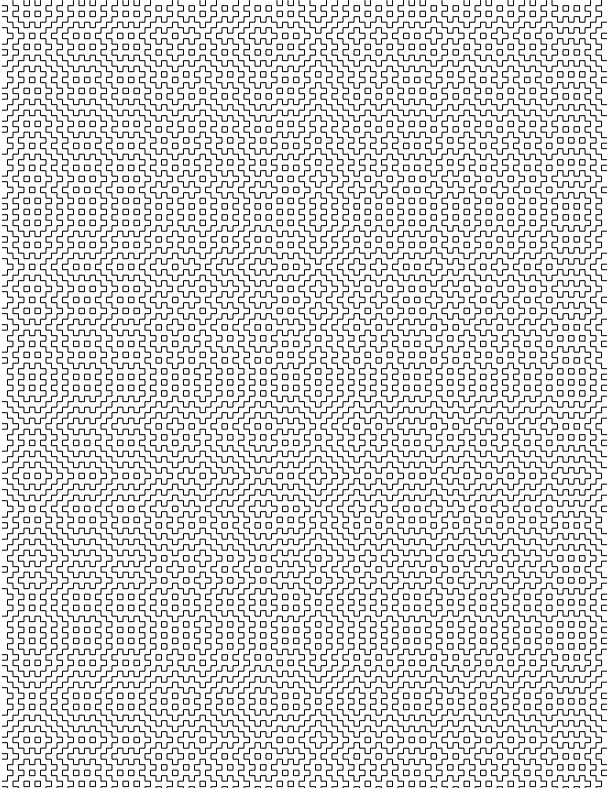
\includegraphics[width=\paperwidth,height=\paperheight]{random_rectangles.png}};

    \node[rounded corners = 8pt, rectangle, inner sep=10pt, fill=white, yshift=8cm] at (current page.center)
              {\makecell{\bfseries\fontsize{40}{60}\selectfont \shadowtext{Terminale option}\\ \bfseries\fontsize{40}{60}\selectfont \shadowtext{Mathématiques expertes}}};
	
	\node[rounded corners = 8pt, rectangle, inner sep=10pt, fill=white, yshift=4cm] at (current page.center)
              {\huge\bfseries Livret d'exercices};

	\node[rounded corners = 8pt, rectangle, inner sep=10pt, fill=white, yshift=3cm] at (current page.center)
              {\large\bfseries 2024-2025};
              
	\node[yshift=-4.5cm] at (current page.center) {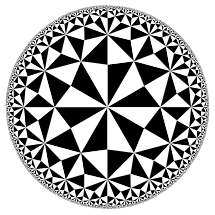
\includegraphics[scale=1]{tessellation.png}};
              
	\node[rounded corners = 8pt, rectangle, inner sep=5pt, fill=white, yshift=-12cm] at (current page.center)
              {\large\bfseries Merlin Olivry};  
\end{tikzpicture}
\end{titlepage}

\renewcommand{\contentsname}{Sommaire}
\hypertarget{sommaire}{}
\tableofcontents
\newpage


\chapter*{Préface}

Chers élèves,

Je suis ravi de vous présenter ce livret d'exercices spécialement conçu pour vous accompagner dans votre parcours en classe de terminale générale avec option mathématiques expertes.\\
Cela fait plusieurs années que j'enseigne les mathématiques, et j'ai souhaité vous offrir un outil complémentaire aux exercices classiques et parfois répétitifs abordés en classe.

\begin{minipage}{0.6\linewidth}
Je précise que je ne prétends à aucune exclusivité quant aux exercices recensés : un exercice ne peut appartenir à personne et vous en trouverez dans ce livret qui sont librement inspirés de sujets de baccalauréats ou d'exercices créés par mes collègues. Mon objectif est avant tout de vous offrir un recueil utile et stimulant pour approfondir vos connaissances.\\

Je revendique cependant la propriété intellectuelle de ce livret en tant que collection d'exercices rédigée et mise en page par mes soins, et toute reproduction devra faire l'objet d'une demande préalable.
\end{minipage}
\begin{minipage}{0.4\linewidth}
\begin{center}
{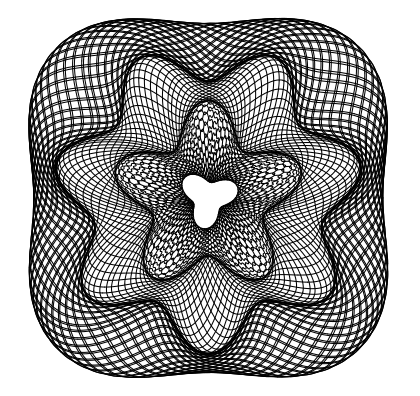
\includegraphics[scale=1]{guilloche.png}}
\end{center}
\end{minipage}


Ce livret est organisé de manière classique par chapitres et sections. Il n'est pas nécessaire de d'avancer linéairement dans son contenu car ces chapitres sont conséquents, et je vous recommande dans la pratique de les séquencer en deux voire trois parties.

J'ai tenté d'ordonner les exercices par ordre croissant de difficulté au sein de chaque section, même si ce classement n'est pas toujours des plus précis. Vous trouverez ainsi des exercices adaptés à différents niveaux, vous permettant de vous exercer en fonction de vos besoin et des défis que vous souhaitez relever.

N’hésitez pas à aborder les exercices avec une attitude exploratoire, car la difficulté n’est pas toujours indiquée et chaque exercice a son propre degré de complexité et demande des initiatives spécifiques.

Je tiens à souligner que ce livret est destiné à être un complément à vos études et non un substitut aux exercices traités en classe. Il a pour but de consolider vos acquis et à parfaire votre maîtrise du programme.

Ne soyez pas découragés si certains exercices vous semblent particulièrement difficiles ; cela ne reflète en aucun cas une incapacité à comprendre le chapitre en question. La persévérance est une clé essentielle pour votre succès, et l'échec fait partie de l'apprentissage.\\

\begin{minipage}{0.4\linewidth}
\begin{center}
{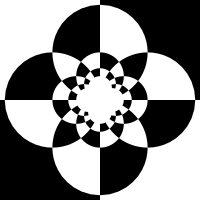
\includegraphics[scale=0.9]{inverse_checker.png}}
\end{center}
\end{minipage}\hfill
\begin{minipage}{0.6\linewidth}
Actuellement, les corrigés des exercices ne sont pas encore disponibles, mais je travaille activement à leur rédaction et je m’efforcerai de les intégrer dans les plus brefs délais.\\
De plus, ce livret est en constante évolution : je prévois d’enrichir son contenu au fil du temps pour mieux répondre à vos besoins et à ceux d'élèves futurs.\\

Je remercie chaleureusement mes élèves qui, chaque jour, résolvent de plus en plus d'exercices et me donnent l'envie de leur en offrir davantage.\\[5pt]
Je tiens à créditer l'ensemble des personnes ayant participé à la lecture, la relecture et la correction de ce livret :
\end{minipage}

\begin{tabular}{p{0.25\linewidth}p{0.25\linewidth}p{0.25\linewidth}p{0.25\linewidth}}
	Jonathan Miron & Victoire Pilon & Thomas Simoes & Estelle Petit
\end{tabular}

Je vous souhaite une excellente utilisation de ce livret et une réussite éclatante dans vos études.\\
Que votre curiosité et vos efforts vous mènent vers de nouveaux horizons mathématiques passionnants !

\vspace{95mm}


Les exercices et questions marquées du symbole $\dur$ sont d'une difficulté supérieure aux attendus de cette année.\\
Les question marquées du symbole \faCalculator~ demandent une réponse aidée par une calculatrice.

Si vous remarquez une coquille ou une erreur, que vous voulez proposer une suggestion d'amélioration ou un nouvel exercice, ou pour toute prise de contact, n'hésitez pas à me contacter à l'adresse
\begin{center}\texttt{merlin.olivry.34@gmail.com}\end{center}

Dernière modification le \today.


%%%%%%%%%%%%%%%%%%%%%%%%%%%%%%%%%%%%%%%%%%%%%%%%%%%%%%%%%%%%%%%%%%%%%%%%%%%%%%%%%%%%%%%%%%%%%%%%%%%%%%%%%%
%%%%%%%%%%%%%%%%%%%%%%%%%%%%%%%%%%%%%%%%%%%%%%%%%%%%%%%%%%%%%%%%%%%%%%%%%%%%%%%%%%%%%%%%%%%%%%%%%%%%%%%%%%
%%%%%%%%%%%%%%%%%%%%%%%%%%%%%%%%%%%%%%%%%%%%%%%%%%%%%%%%%%%%%%%%%%%%%%%%%%%%%%%%%%%%%%%%%%%%%%%%%%%%%%%%%%
%%%%%%%%%%%%%%%%%%%%%%%%%%%%%%%%%%%%%%%%%%%%%%%%%%%%%%%%%%%%%%%%%%%%%%%%%%%%%%%%%%%%%%%%%%%%%%%%%%%%%%%%%%
%%%%%%%%%%%%%%%%%%%%%%%%%%%%%%%%%%%%%%%%%%%%%%%%%%%%%%%%%%%%%%%%%%%%%%%%%%%%%%%%%%%%%%%%%%%%%%%%%%%%%%%%%%
\titleformat{\chapter}
  {\gdef\chapterlabel{}
   \normalfont\Huge\bfseries\scshape}
  {\gdef\chapterlabel{Chapitre \no\thechapter}}{0pt}
  {\begin{tikzpicture}[remember picture,overlay]
  	\node[opacity=0.2,inner sep=0pt] at (current page.center)	{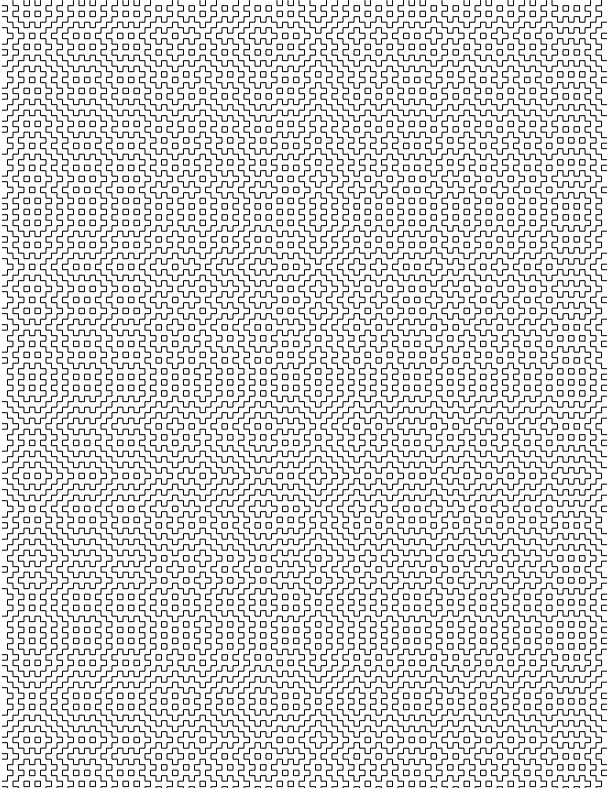
\includegraphics[width=\paperwidth,height=\paperheight]{random_rectangles.png}};
    \node[yshift=-50mm] at (current page.north west)
      {\begin{tikzpicture}[remember picture, overlay]
        \draw (0,0) (\paperwidth,3cm);
        \node[rounded corners = 5pt, anchor=west,xshift=.1\paperwidth,rectangle, inner sep=11pt, fill=black]
              {\makecell{\color{white}\chapterlabel \\ \color{white}#1}};
       \end{tikzpicture}
      };
   \end{tikzpicture}
 }
\titlespacing{\chapter}{0pt}{50pt}{-40pt}
%%%%%%%%%%%%%%%%%%%%%%%%%%%%%%%%%%%%%%%%%%%%%%%%%%%%%%%%%%%%%%%%%%%%%%%%%%%%%%%%%%%%%%%%%%%%%%%%%%%%%%%%%%
%%%%%%%%%%%%%%%%%%%%%%%%%%%%%%%%%%%%%%%%%%%%%%%%%%%%%%%%%%%%%%%%%%%%%%%%%%%%%%%%%%%%%%%%%%%%%%%%%%%%%%%%%%
%%%%%%%%%%%%%%%%%%%%%%%%%%%%%%%%%%%%%%%%%%%%%%%%%%%%%%%%%%%%%%%%%%%%%%%%%%%%%%%%%%%%%%%%%%%%%%%%%%%%%%%%%%
%%%%%%%%%%%%%%%%%%%%%%%%%%%%%%%%%%%%%%%%%%%%%%%%%%%%%%%%%%%%%%%%%%%%%%%%%%%%%%%%%%%%%%%%%%%%%%%%%%%%%%%%%%
%%%%%%%%%%%%%%%%%%%%%%%%%%%%%%%%%%%%%%%%%%%%%%%%%%%%%%%%%%%%%%%%%%%%%%%%%%%%%%%%%%%%%%%%%%%%%%%%%%%%%%%%%%


\chapter{Nombres complexes}


\newpage



\section{Calcul et forme algébrique}

\subsection{Puissances de $i$}
\begin{enumerate}
    \item Déterminer la valeur de $\frac{1}{i}$
    \item Calculer $i^2, i^3, i^4$ et $i^5$
    \item En déduire la valeur de $i^{2023}$ et celle de $i^{123456}$
    \item Déterminer les entiers naturels $n$ pour lesquels $\sommek{1}{n}i^k =0$
\end{enumerate}



\subsection{Forme algébrique de sommes et produits}
Donner la forme algébrique chacun des nombres suivants, en précisant la partie réelle et la partie imaginaire :\\
\renewcommand{\arraystretch}{1.5}
\begin{tabular}{p{0.33\textwidth} p{0.33\textwidth} p{0.33\textwidth}}
    $z_1=(2i-5)-(i+4)$ & $z_2=(1-i)(3+2i)$ & $z_3=i(2-i)-4(i^2+3i)$ \\
    $z_4=i(2-2i)^2$ & $z_5=(7i+2)(i-3)^2$ & $z_6=(1-i)^3$ \\
    $z_7=(i+\sqrt{3})^3$ & $z_8=(1+i)^4$ & $z_9=(\sqrt{2}+i\sqrt{6})^5$
\end{tabular}



\subsection{Forme algébrique de quotients}
Donner la forme algébrique de chacun des quotients suivants :\\
\renewcommand{\arraystretch}{1.5}
\begin{tabular}{p{0.33\textwidth} p{0.33\textwidth} p{0.33\textwidth}}
    $z_1=\frac{1}{1+i}$ & $z_2=\frac{-2}{i+\sqrt{2}}$ & $z_3=\frac{3+i}{1-2i}$ \\
    $z_4=\frac{(2i-3)^2}{i+4})$ & $z_5=\left(\frac{3+i}{1+2i}\right)^2$ & $z_6=\frac{\sqrt{2}+i\sqrt{6}}{(\sqrt{6}+\sqrt{2})+i(\sqrt{6}-\sqrt{2})}$ \\
\end{tabular}



\subsection{Équations dans $\CC$}
Résoudre dans $\CC$ les équations suivantes :\\
\begin{tabular}{p{0.3\textwidth} p{0.3\textwidth} p{0.3\textwidth}}
    a) $z+2i=iz-1$ & b) $(3i+2)(z-i)=i$ & c) $(3-i)z+2=(2-1)z+i$\\
    d) $(4-2i)z=(i+5)z^2$ & e) $(z+i)^2=2iz$ & f) $\frac{1}{z}=-5+3i$ \\
    g) $\frac{z}{z-2i}=3+i$ & h) $\frac{iz}{i-z}=\frac{1}{1-i}$ & k) $\frac{z+2i}{2z+1}=1+i$
\end{tabular}


\subsection{Équations avec conjugué}
Résoudre dans $\CC$ les équations suivantes : \\
\begin{tabular}{p{0.4\textwidth} p{0.4\textwidth}}
    a) $ 2z+i=\barre{z}$ & b) $2\barre{z}-z=3i+2$ \\
    c) $\barre{z}-2z=3i+2$ & d) $(z-1)(\barre{z}-i)=1+i$ 
\end{tabular}



\subsection{Changement de variable}
Pour $z\in\CC\backslash\{-1\}$ on pose $Z=\frac{z}{1+z}$
\begin{enumerate}
	\item Montrer que $Z$ est réel si et seulement si $z$ est réel.
	\item Montrer que si $z$ a une partie réelle strictement positive, alors $Z$ n'est pas un imaginaire pur.
\end{enumerate}



\subsection{Transformation plus compliquée}
Pour $z\in\CC$ non nul on note $z'=z-\frac{1}{z}$

Montrer que $z'$ est réel si et seulement si $z$ est réel.



\subsection{Vrai / Faux}
Déterminer si les affirmations suivantes sont vraies ou fausses :
\begin{enumerate}\setlength{\itemsep}{0.5mm}
	\item $\Reel(z+\barre{z})=\Imag(z-\barre{z})$
    \item $\left(\Reel(1+i)\right)^2=\Reel\left((1+i)^2\right)$
    \item $\Reel(z^2)=\Reel(z)^2 \Leftrightarrow z=\barre{z}$
    \item $\Imag\left(\frac{1}{z}\right)=\dfrac{\Imag(z)}{z\barre{z}}$
    \item $\Imag(z)+i\Reel(z)=i\barre{z}$
    \item $\Imag(\Reel(z))=\Reel(\Imag(z)) \Leftrightarrow z\in\RR$
\end{enumerate}



\section{Polynômes dans $\CC$}

\subsection{Sur l'intérêt des nombres complexes}
\begin{enumerate}
    \item  Résoudre dans $\CC$ les équations suivantes :
    
    \begin{tabular}{p{0.33\textwidth} p{0.33\textwidth} p{0.33\textwidth}}
        a) $z^2-2z+2=0$ & b) $z^2+6z+13=0$ & c) $2z^2-3z+4=0$
    \end{tabular}

    \item Résoudre dans $\CC$ les systèmes d'équations suivants :

    \renewcommand{\arraystretch}{1}
    \begin{tabular}{p{0.33\textwidth} p{0.33\textwidth} p{0.33\textwidth}}
        $\accol{z+w=2\\z\times w=3}$ & $\accol{z(w+1)=3\\w(z+1)=2}$ & $\accol{z^2+2w\,^2=1\\2z+w=3}$ 
    \end{tabular}
\end{enumerate}



\subsection{Polynôme de dergé 3}
On considère le polynôme $R:z\mapsto z^3+z-10$
\begin{enumerate}
	\item Déterminer $x_0$ une racine réelle évidente de $R$
	\item Déterminer un polynôme $P$ de degré 2 tel que $R(z)=(z-x_0)P(z)$
	\item Déterminer l'ensemble des racines de $R$
\end{enumerate}


\subsection{Coefficients complexes, racines réelles ?}
Pour tout $z\in\CC$  on pose $\mu(z)=2z^3+(3+6i)z^2+(1+9i)z+3i$
\begin{enumerate}
	\item Montrer que le polynôme $\mu$ admet une racine imaginaire pure notée $z_0$
	\item Factoriser $\mu(z)$ par $(z-z_0)$
	\item Résoudre alors l'équation $\mu(z)=0$
\end{enumerate}



\subsection{Degré 3 à coefficients complexes}
On considère le polynôme $P$ défini par $P(z)=z^3-(6+2i)z^2+(10+12i)z-20i$
\begin{enumerate}
    \item Montrer que le polynôme $P$ admet une racine $z_1$ qui est un imaginaire pur.
    \item Déterminer un polynôme $Q$ tel que $P(z)=(z-z_1)Q(z)$
    \item Résoudre $P(z)=0$
\end{enumerate}



\subsection{Polynôme de degré 4}
On considère le polynôme $P$ défini par $P(z)=z^4-iz^3+8z-8i$
\begin{enumerate}
	\item Montrer que $P$ admet une racine réelle $z_1$
	\item Montrer que $P$ admet une racine imaginaire pure $z_2$
	\item En déduire que $P(z)=\left[z^2+(2-i)z-2i\right]Q(z)$ avec $Q$ un polynôme de degré 2.
	\item Donner toutes les racines de $P$ sous forme exponentielle. 
\end{enumerate}



\subsection{Racines de $i$}
\begin{enumerate}
    \item Déterminer les \og racines carrées \fg du nombre $i$, c'est à dire les nombre $\zC$ tels que $z^2=i$
    \item Déterminer les \og racines cubiques \fg du nombre $i$, c'est à dire les nombres $w\in\CC$ tels que $w^3=i$
\end{enumerate}



\subsection{Racines carrées complexes}
Déterminer les racines carrées complexes des nombres suivants :

\begin{tabular}{p{0.3\textwidth} p{0.3\textwidth}p{0.3\textwidth}}
    $z_1=2-2i$ & $z_2=3+4i$ & $z_3 = 5i-8$\\
    $z_4=\frac{1+i}{i-2}$ & $z_5=(3-2i)^5$ & $z_6=\frac{i\sqrt{2}+1}{\sqrt{3}-i}$
\end{tabular}



\subsection{Trinôme à coefficients complexes}
L'objectif de cet exercice est de résoudre l'équation $(E):z^2+(1-3i)z-4-3i=0$ en applicant la méthode du discriminant complexe.
\begin{enumerate}
    \item En posant $a,b$ et $c$ les coefficients des degrés 2, 1 et 0 de $z$ dans $(E)$, calculer $\Delta_E=b^2-4ac$
    \item Déterminer $\delta_1$ et $\delta_2$ les deux racines carrées complexes de $\Delta_E$
    \item Calculer $z_1=\frac{-b+\delta_1}{2a}$ et $z_2=\frac{-b+\delta_2}{2a}$
    \item Vérifier que $z_1$ et $z_2$ sont solutions de $(E)$
\end{enumerate}



\subsection{On recommence}
En utilisant la même méthode que dans l'exercice précédent, résoudre dans $\CC$ l'équation \[2iz^2-(5+i)z+5-5i=0\]



\section{Formes trigonométriques et exponentielles}

\subsection{Calcul de modules}
Calculer le module des nombres suivants :\\
\begin{tabular}{p{0.33\textwidth} p{0.33\textwidth} p{0.33\textwidth}}
	$z_1=i+2$ & $z_2=i\sqrt{3}-1$ & $z_3=\frac{4}{i}$ \\
    $z_4=(5+2i)(\sqrt{3}-i\sqrt{6})$ & $z_5=\left(\frac{\sqrt{6}-i\sqrt{2}}{2}\right)^2$ & $z_6=\frac{(2-i)^5}{(1+2i)^4}$
\end{tabular}



\subsection{Peu de calcul}
On pose $z=2i-1$ et $w=\sqrt{3}+i$
\begin{enumerate}
	\item Déterminer le module de $z$ et de $w$
	\item Calculer les modules des nombres suivants en utilisant les résultats de la question précédente :\\[5pt]
$3+i\sqrt{3}$ \quad\quad ; \quad $\frac{i+\sqrt{3}}{1-2i}$ \quad\quad ; \quad $\frac{i}{2}-\frac{1}{4}$ \quad\quad ; \quad $(\sqrt{3}-i)^5$ 
\end{enumerate}



\subsection{Encore celui-là ?}
Pour $z\in\CC$ non nul on note $z'=z-\frac{1}{z}$

À quelle condition sur $z$ le nombre $z'$ est-il imaginaire pur ?



\subsection{Module imaginaire}
Soit $z\in\CC\setminus\{1\}$\\
Montrer que $\frac{1+z}{1-z}$ est un imaginaire pur si et seulement si $\abs{z}=1$



\subsection{Forme trigonométrique}
Donner la forme trigonométrique, puis la forme exponentielle de chacun des nombres suivants :\\
\begin{tabular}{p{0.3\textwidth} p{0.3\textwidth} p{0.3\textwidth}}
    $z_1=1+i\sqrt{3}$ & $z_2=1-i$ & $z_3= 9i-3\sqrt{3}$ \\
    $z_4=i$ & $z_5=-5$ & $z_6=\sqrt{2}(i-1)$ \\
    $z_7=\frac{-i\sqrt{2}}{1+i}$ & $z_8=\sin(\theta)+i\cos(\theta)$ 
\end{tabular}



\subsection{Forme exponentielle}
Déterminer la forme exponentielle de chacun des nombres complexes suivants : \\
\renewcommand{\arraystretch}{1.7}
\begin{tabular}{p{0.3\textwidth} p{0.3\textwidth} p{0.2\textwidth}}
    $z_1=(1+i\sqrt{3})(2-2i)$ & $z_2=(1+i)^5$ & $z_3=\frac{3-i\sqrt{3}}{4+4i}$ \\
    $z_4=\frac{(i-\sqrt{3})^5}{(i-1)^4}$ & $z_5=\frac{1+i\sqrt{3}}{\sqrt{2}+\sqrt{6}+i(\sqrt{6}-\sqrt{2})}$ & $z_6=\frac{i-1-\sqrt{3}(1+i)}{2+2i}$
\end{tabular}




\subsection{Écriture piégeuse}
On pose $z_1=2e^{i\frac{\pi}{3}}, \quad z_2=ie^{i\frac{\pi}{4}}$ \, et \, $z_3=-3e^{i\frac{\pi}{6}}$
\begin{enumerate}
	\item Donner la forme exponentielle de $z_2$ et $z_3$
	\item Calculer sous forme exponentielles les nombres suivants : \\
        $z_1z_2$ ~~~~;~~~~ $z_1z_3$~~~~;~~~~$\frac{z_2z_3}{z_1}$~~~~;~~~~$\frac{z_3\,^3}{z_2\,^2}$
\end{enumerate}



\subsection{Retour à la forme algébrique}
Donner la forme algébrique des nombres complexes suivants :

\begin{tabular}{p{0.3\textwidth} p{0.3\textwidth} p{0.3\textwidth}}
    $z_1=2e^{i\frac{\pi}{3}}$ & $z_2=e^{i\frac{\pi}{4}}\times (e^{i\frac{2\pi}{6}})$ & $z_3=\frac{3e^{2i\frac{\pi}{3}}}{5e^{-i\frac{\pi}{6}}}$ \\
    $z_4=\frac{e^{i\frac{\pi}{3}}}{2e^{i\frac{7\pi}{12}}}$ & $z_5=\left(e^{i\frac{\pi}{4}}\right)^{2023}$ & $z_6 = (2-2i)^5$ \\
    $z_7=\frac{(1+i)^{2000}}{(i-\sqrt{3})^{1000}}$
\end{tabular}



\subsection{Une nouvelle valeur trigonométrique}
On pose $z_1=1+i\sqrt{3}$ et $z_2=1+i$
\begin{enumerate}
    \item Donner la forme algébrique de $\frac{z_1}{z_2}$
    \item Donner la forme exponentielle de $\frac{z_1}{z_2}$
    \item En déduire la valeur de $\cos(\frac{\pi}{12})$ et de $\sin(\frac{\pi}{12})$, puis de $\cos(\frac{5\pi}{12})$ et de $\sin(\frac{5\pi}{12})$
\end{enumerate}



\subsection{Puissances de nombres complexes}
\begin{enumerate}
    \item Déterminer les entiers $n\in\ZZ$ tels que $(2i+2)^n$ soit un imaginaire pur.
	\item Déterminer les entiers $n\in\ZZ$ tels que $(3-i\sqrt{3})^n$ soit un nombre réel.
\end{enumerate}



\subsection{Linéarisation}
\begin{enumerate}
	\item Linéariser $\sin^3(x)$
	\item Linéariser $\cos^4(x)$
	\item Linéariser $\sin^2(x)\cos^3(x)$
\end{enumerate}



\subsection{Puissances conjuguées}
\begin{enumerate}
    \item Montrer que $(1+i)^n+(1-i)^n=2\sqrt{2^n}\cos\left(\frac{\pi n}{4}\right)$
    \item Généraliser en montrant que $z^n+\barre{z}^n=2\abs{z}^n\cos(n\arg(z))$
\end{enumerate}



\section{Application à la géométrie}

\subsection{Étude d'un triangle}

On munit le plan complexe du repère orthonormé $\Ouv$ et on considère les points A, B et C d'affixes respectives $z_A=-3+4i$, $z_B=2+3i$ et $z_C=-4-i$ \\
Déterminer la nature du triangle $ABC$.



\subsection{Alignement}
Soient $A(z_A)$, $B(z_B)$ et $C(z_C)$ trois points distincs du plan complexe.

Montrer que $A$, $B$ et $C$ sont aligné si et seulement si $\arg\left(\frac{z_A-z_B}{z_A-z_C}\right)=0 \left[\pi\right]$



\subsection{Alignement}
On munit le plan complexe du repère orthonormé $\Ouv$. Pour tout complexe $z$ non nul on considère le point $M$ d'affixe $z$ et le point $M'$ d'affixe $-\frac{1}{\barre{z}}$ \\
Montrer que $M$, $O$ et $M'$ sont alignés.




\subsection{Racines rectangles}
Soit le polynôme $P:z\mapsto z^3-3z^2+9z+13$

Démontrer que les points dont les affixes sont les racines de $P$ forment un triangle isocèle rectangle dans le plan complexe.


\subsection{Une suite de points}

On considère la suite $(z_n)_{\nN}$ définie par $z_n=(\sqrt{3}-i)^n$. \\
On munit le plan complexe du repère orthonormé $\Ouv$ et on note $M_n$ le point d'affixe $z_n$
\begin{enumerate}
    \item Montrer que $M_n$, $O$ et $M_{n+6}$ sont alignés pour tout $n$ naturel.
    \item Montrer que le triangle $M_nOM_{n+3}$ est rectangle pour tout $n$ naturel.
\end{enumerate}



\subsection{Inscrits dans un cercle}
On munit le plan complexe du repère orthonormé $\Ouv$ et on considère les points A, B, C et D d'affixes respectives $z_A=-1+3i$, $z_B=2+4i$, $z_C=1-3i$ et $z_D=4+3i$

\begin{enumerate}
    \item Déterminer la nature du triangle $BCD$
    \item Montrer que les points $A$, $B$, $C$ et $D$ appartiennent tous à un même cercle $\mathscr{C}$ dont on donnera le centre $P$, le rayon $r$ et une équation.
    \item Déterminer l'affixe $z_E$ du point $E\in\mathscr{C}$ tel que $APE$ soit un triangle rectangle et $\Reel{z_E}>0$ 
\end{enumerate}



\subsection{Transformation du plan}
On munit le plan complexe du repère orthonormé $\Ouv$ et à tout point $M(z)$ avec $z\neq3-i$ on associe le point $M'(z')$ tel que $z'=\frac{z-2i}{z-3+i}$\\
On dira que $M'$ est l'image du point $M$.
\begin{enumerate}
	\item Déterminer sous forme algébrique l'affixe de l'image du point $M(i)$
	\item Peut-on trouver un point $M$ dont l'image a une affixe égale à $1+i$ ?
	\item Déterminer et représenter l'ensemble des points $M$ pour lesquels $z'$ est un nombre réel.
	\item Déterminer et représenter l'ensemble des points $M$ pour lesquels $\abs{z'}=1$
	\item Déterminer et représenter l'ensemble des points $M$ pour lesquels $z'$ est un imaginaire pur.
\end{enumerate}



\subsection{Fonction complexe}
On définit la fonction $f:z\mapsto\frac{z-1+2i}{2z-3i}$
\begin{enumerate}
	\item Le nombre $i$ admet-il un antécédent par la fonction $f$ ?
	\item Déterminer l'ensemble des $\zC$ tels que $f(z)\in\RR$ puis représenter cet ensemble sur le plan complexe.
	\item Déterminer l'ensemble des $\zC$ tels que $f(z)\in i\RR$ puis représenter cet ensemble sur le plan complexe. 
	\item Déterminer l'ensemble des $\zC$ tels que $\abs{f(z)}=1$ puis représenter cet ensemble sur le plan complexe. 
\end{enumerate}




\subsection{Ensembles de points}
Déterminer et représenter l'ensemble des points $M$ du plan complexe dont l'affixe $z$ vérifie les équations suivantes :

\begin{tabular}{p{0.4\textwidth} p{0.4\textwidth}}
    a) $\abs{z-3i} = \abs{z+i-2} $ & b) $\abs{z+2+1}=\abs{2i+1} $ \\
    c) $\abs{\barre{z}+i}=\abs{z+1} $ & d) $\abs{\frac{z-3i}{iz+2+i}} = 1$ \\
    e) $\arg(z)=\frac{\pi}{3} \quad\pi]$ & f) $\arg(z)=\arg(-\barre{z}) \quad[2\pi]$ \\
    g) $\arg(z-2+3i)=\frac{\pi}{4} \quad[2\pi]$ & h) $\arg(z+4i)=\arg(z-2-i) \quad[\pi]$ \\
    i) $\arg(z+4i)=\arg(z-2-i)\quad [2\pi]$ & j) $\abs{1+z}=2\abs{z}$ \\     
\end{tabular}



\section{Sur les racines n-ièmes}

\subsection{Équations simples}
Résoudre dans $\CC$ les équations suivantes :

\begin{tabular}{p{0.28\textwidth} p{0.28\textwidth} p{0.28\textwidth}}
    a) $z^5=i$ & b) $z^4=2\sqrt{2}(1+i)$ & c)  $z^6=-8i$ \\
    d) $z^6=\frac{4}{1-1\sqrt{3}}$ & e) $z^4=\frac{16\sqrt{2}}{1+i}$ & f) $z^4=\frac{(3+i\sqrt{3})^3}{(1-i)^2}$
\end{tabular}


\subsection{Ça y ressemble}
Résoudre dans $\CC$ les équations suivantes :

\begin{tabular}{p{0.28\textwidth} p{0.28\textwidth} p{0.28\textwidth}}
    a)$\left(\frac{z+3i}{z-2}\right)^4=1$ & b) $\left(\frac{z-1}{z-i}\right)^3=-8$  & c) $27(z-1)^6+(z+1)^6=0$
\end{tabular}


\subsection{Périmètres}
\begin{enumerate}
    \item Calculer le périmètre d'un hexagone régulier inscrit dans un cercle de rayon 1.
    \item Calculer le périmètre d'un dodécagone régulier inscrit dans un cercle de rayon 2.
\end{enumerate}



\subsection{Somme et produit}
\begin{enumerate}
	\item Que vaut la somme de toutes les racines $n$-ièmes de l'unité ?
	\item Que vaut le produit de toutes les racines $n$-ièmes de l'unité ?
\end{enumerate}



\subsection{Sommes non complètes}
On considère $w=e^{i\frac{2\pi}{5}}$ puis on pose $A=w+w^4$ et $B=w^2+w^3$
\begin{enumerate}
	\item Montrer que $A+B=-1$
	\item Montrer que $AB=-1$
	\item En déduire que $A^2+A-1=0$
	\item En déduire la valeur de $A$, puis celle de $B$
	\item Déterminer alors $\cos\left(\frac{2\pi}{5}\right)$ et $\sin\left(\frac{2\pi}{5}\right)$
	\item En déduire les valeurs de $\cos\left(\frac{\pi}{5}\right)$ et $\sin\left(\frac{\pi}{5}\right)$
\end{enumerate}



\subsection{Somme de modules}
On note $\mathbb{U}_n$ l'ensemble des racines $n$-ièmes de l'unité.\\
L'objectif de l'exercice est de calculer $S_n=\somme{z\in\mathbb{U}_n}{}\abs{1-z}$
\begin{enumerate}
	\item Justifier que $S_n=\sommek{0}{n-1}\abs{1-e^{i\frac{2k\pi}{n}}}$
	\item \begin{enumerate}
		\item Montrer que $\abs{1-e^{2ix}}^2=2\left(1-\cos(2x)\right)$ \quad $\forall\xR$
		\item En déduire que $\abs{1-e^{i\frac{2k\pi}{n}}}=2\sin\left(\frac{k\pi}{n}\right)$
	\end{enumerate}
	\item \begin{enumerate}
		\item Montrer que $S_n=-i\sommek{0}{n-1}\left(e^{i\frac{k\pi}{n}}-e^{-i\frac{k\pi}{n}}\right)$
		\item En déduire que $S_n=2i\left(\frac{1}{1-e^{-i\frac{\pi}{n}}}-\frac{1}{1-e^{i\frac{\pi}{n}}}\right)$
	\end{enumerate}
	\item Montrer que $S_n=\frac{2\sin\left(\frac{\pi}{n}\right)}{1-\cos\left(\frac{\pi}{n}\right)}$
	\item Montrer alors que $S_n=\frac{2}{\tan\left(\frac{\pi}{2n}\right)}$
	\item Déterminer $\limn S_n$\\
	Aurait-on pu prédire ce résultat géométriquement ?
\end{enumerate}




\section{Exercices supplémentaires}

\subsection{Module et argument de somme et différence}

On considère $z=re^{i\theta}$ et $w=r'e^{i\theta'}$ deux nombres complexes non nuls. \\
Montrer que $\abs{z+w}=\abs{z-w}\Longleftrightarrow \theta=\theta'+\frac{\pi}{2} [\pi]$



\subsection{Étude d'une suite}

On définit la suite $(z_n)_{\nN}$ par $\defsuitez{z_0=i}{(1-i)z_n+2}$
\begin{enumerate}
    \item On pose $w_n=z_n+2i$ pour tout $\nN$ \\
    Montrer que $w_{n+1}=(1-i)w_n$ pour tout $\nN$
    \item Montrer par récurrence que $w_n=3i(1-i)^n$
    \item En déduire l'expression de $z_n$ en fonction de $n$
    \item Montrer que $z_n\neq0$ pour tout $\nN$
    \item Montrer que $z_n$ n'est jamais un nombre réel.
    \item Déterminer pour quels $\nN$ le nombre $z_n$ est un imaginaire pur.
\end{enumerate}


%%%%%%%%%%%%%%%%%%%%%%%%%%%%%%%%%%%%%%%%%%%%%%%%%%%%%%%%%%%%%%%%%%%%%%%%%%%%%%%%%%%%%%%%%%%%%%%%%%%%%%%%%%
%%%%%%%%%%%%%%%%%%%%%%%%%%%%%%%%%%%%%%%%%%%%%%%%%%%%%%%%%%%%%%%%%%%%%%%%%%%%%%%%%%%%%%%%%%%%%%%%%%%%%%%%%%
%%%%%%%%%%%%%%%%%%%%%%%%%%%%%%%%%%%%%%%%%%%%%%%%%%%%%%%%%%%%%%%%%%%%%%%%%%%%%%%%%%%%%%%%%%%%%%%%%%%%%%%%%%
%%%%%%%%%%%%%%%%%%%%%%%%%%%%%%%%%%%%%%%%%%%%%%%%%%%%%%%%%%%%%%%%%%%%%%%%%%%%%%%%%%%%%%%%%%%%%%%%%%%%%%%%%%
%%%%%%%%%%%%%%%%%%%%%%%%%%%%%%%%%%%%%%%%%%%%%%%%%%%%%%%%%%%%%%%%%%%%%%%%%%%%%%%%%%%%%%%%%%%%%%%%%%%%%%%%%%

\chapter{Arithmétique des nombres entiers}
\newpage

\section{Divisibilité dans $\ZZ$}

\subsection{Parité}
\begin{enumerate}
    \item Montrer que $n$ et $n^2$ sont toujours de même parité
    \item Montrer par récurrence sur $k$ que $n$ et $n^k$ sont toujours de même parité
\end{enumerate}



\subsection{Divisibilité dans $\NN$}
Déterminer les entiers naturels $n$ tels que :

\renewcommand{\arraystretch}{1.2}
\begin{tabular}{p{0.33\linewidth} p{0.33\linewidth} p{0.33\linewidth}}
	a) $n-4\vert 3n-17$ & b) $n-1 \vert n+6$ & c) $n+2 \vert 2n-1$ \\
	d) $n+1 \vert n^2$ & e) $n+2 \vert 2n^2+3$ & f) $n-3 \vert n^3-3$
\end{tabular} 
        
        
        
\subsection{Divisibilité dans $\ZZ$}
Déterminer les entiers relatifs $n$ tels que :

\renewcommand{\arraystretch}{1.2}
\begin{tabular}{p{0.33\linewidth} p{0.33\linewidth} p{0.33\linewidth}}
	a) $n \vert n+8$ & b) $n \vert n^2+2n+3$ & c) $n-3 \vert n^2+2n-1$ \\
	d) $n+3 \vert n^3+3$ & e) $2n+1 \vert 4n^2+4n+3$ & f) $3n-2 \vert 6n^3$
\end{tabular} 



\subsection{Des fractions ???}
\begin{enumerate}
	\item Déterminer les entiers relatifs $k$ tels que $\frac{12k+7}{3k+1}\in\NN$ 
	\item Déterminer les entiers naturels $m$ tels que $\frac{5m-1}{2m+3}\in\ZZ$
\end{enumerate}



\subsection{Puissances de n}
\begin{enumerate}
    \item \begin{enumerate}
        \item Montrer que $n^3-n$ est un multiple de 3 pour tout $\nN$
        \item Montrer que c'est également un multiple de 2
    \end{enumerate}
    \item Pour $\nN$, on pose $B_n=n^4-3n^3-n^2+3n+1$
    \begin{enumerate}
        \item Montrer que $B_n$ est toujours un nombre impair
        \item Résoudre alors $n(n+3)\vert B_n$ dans $\NN$
    \end{enumerate}
\end{enumerate}



\subsection{Équations dans $\ZZ$}
Résoudre dans $\ZZ$ les équations suivantes :

\begin{tabular}{p{0.33\linewidth} p{0.33\linewidth} p{0.33\linewidth}}
    a) $x^3+2x+3=0$ & b) $2x^2+xy=35$ & c) $x^2-y^2=17$ \\
    d) $x^2-y^2=2023$ & e) $x^2=17+4y^2$ & f) $xy = 2x +3y$ \\
    g) $\frac{1}{x}+\frac{1}{y}=\frac{1}{5}$ & h) $x^2+6x-y^2=0$ & i) $x^2-y^2+4x+4y=0$ \\
\end{tabular}



\subsection{n en puissance}
Démontrer par récurrence et pour tout $\nN$ les affirmations suivantes :
\begin{enumerate}
    \item[a)] 3 divise le nombre $2^{n+1}+5^n$
    \item[b)] $3^{2n}-2^n$ est un multiple de 7
    \item[c)] 5 divise $2^{2n+1}+3^{2n+1}$
    \item[d)] $2^{4n}-7^n$ est un multiple de 9
\end{enumerate}



\section{Division euclidienne}

\subsection{Rappel}
\begin{enumerate}
	\item Déterminer le reste dans la division euclidienne de 1023 par 47.
	\item Déterminer le reste dans la division euclidienne de 2048 par 81.
\end{enumerate}



\subsection{Division par 6}
Déterminer tous les entiers relatifs ayant un reste et un quotient égal dans la division euclidienne par 6.



\subsection{Réduction du diviseur}
Soit $a$ un entier naturel dont le reste dans la division euclidienne par 24 vaut 13.\\
Quel est le reste dans la division euclidienne de $a$ par 6 ? Et par 8 ?



\subsection{Puis augmentation}
On considère $M$ un entier naturel dont le reste dans la division euclidienne par 6 vaut 3.\\
Quels sont les restes possibles dans la division euclidienne de $M$ par 30 ?



\subsection{Déterminer le reste}
\begin{enumerate}
	\item Déterminer selon la valeur de $\nN$ la reste dans la division euclidienne de $n^2+2n+4$ par $n^2+n$
	\item Déterminer selon la valeur de $\nN$ la reste dans la division euclidienne de $2n^2+5n-1$ par $n+3$ 
\end{enumerate}



\subsection{En connaissant le reste}
Déterminer tous les entiers naturels $k$ pour lesquels le reste dans la division euclidienne de $(2k+1)^2$ par $k^2+k$ vaut $3k-2$



\subsection{Divisions impossibles}
Démontrer qu'il n'existe aucun nombre entier ayant un reste de 5 après division par 6, et un reste de 2 après division par 14.



\subsection{Le reste reste le même}
\begin{enumerate}
	\item Déterminer les entiers naturels $n$ ayant le même reste que $2-n$ dans la division euclidienne par 7.
	\item Déterminer les entiers naturels $n$ ayant le même reste que leur double dans la division euclidienne par 5.
\end{enumerate}


\section{Congruences dans $\ZZ$}

\subsection{Tableaux de congruences}
Compléter les tableaux de congruence suivants :
    
    \begin{minipage}{0.5\textwidth}
    \setlength{\tabcolsep}{15pt}
        \begin{tabular}{|c|c|c|c|c|c|c|} \hline
        $n$&0&1&2&3&4&5 \\ \hline
        $2n^2$& & & & & & \\ \hline
      \end{tabular}
      
      \smallskip
      \centering \small Modulo 6
    \end{minipage}
    \begin{minipage}{0.5\textwidth}
    \setlength{\tabcolsep}{15pt}
        \begin{tabular}{|c|c|c|c|c|c|} \hline
        $n$&0&1&2&3&4 \\ \hline
        $4-n^3$& & & & & \\ \hline
      \end{tabular}
      
      \smallskip
      \centering \small Modulo 5
    \end{minipage}\\[15pt]

    \begin{minipage}{\textwidth}
    \setlength{\tabcolsep}{24pt}
        \begin{tabular}{|c|c|c|c|c|c|c|c|c|} \hline
        $n$&0&1&2&3&4&5&6&7 \\ \hline
        $3n$& & & & & & & & \\ \hline
        $n^2$& & & & & & & & \\ \hline
        $3n+n^2$& & & & & & & & \\ \hline
      \end{tabular}
      
      \smallskip
      \centering \small Modulo 8
    \end{minipage}\\[5pt]



\subsection{Dresser un tableau}
Dresser le tableau de congruences modulo $a$ des expressions suivantes :

\begin{tabular}{p{0.25\linewidth} p{0.2\linewidth} |p{5mm} p{0.2\linewidth} p{0.1\linewidth}}
	a) $n^2+n-1$ & $a=4$ && b) $n^3-2n$ & $a=5$ \\
	c) $n(2n+1)(2n+2)$ & $a=7$ && d) $(n^2-3n)^2$ & $a=6$
\end{tabular}



\subsection{Impossibles équations}
\begin{enumerate}
    \item En raisonnant modulo 2, montrer que l'équation : $3n^3-2n^2-n=1$ n'a pas de solutions dans $\NN$
    \item En raisonnant modulo 6, montrer que l'équation : $5n^3-14n=112$ n'a pas de solutions dans $\ZZ$
    \item En raisonnant modulo 4, montrer que l'équation $5x^2-3y^2=1$ n'a aucune solution dans $\ZZ$
\end{enumerate}



\subsection{Retour en arrière}
Répondre aux questions des exercices 2.1.7, 2.2.7 et 2.2.8 avec la notion de congruence dans $\ZZ$, sans raisonnement par récurrence ni disjonction de cas.



\subsection{Le chiffre de l'année}
\begin{enumerate}
    \item Déterminer le reste de la division euclidienne de 2023 par 7
    \item Déterminer le reste de la division euclidienne de $7^{2023}$ par 6
    \item Déterminer le reste de la division euclidienne de $7^{2023}$ par 8
    \item Déterminer chiffre des unités de $7^{2023}$
\end{enumerate}



\subsection{De grands multiples}
\begin{enumerate}
    \item Déterminer le reste dans la division euclidienne de 512 par 19
    \item Déterminer les valeurs possibles pour le reste dans la division euclidienne de $2^{9m}$ par 19
    \item En déduire alors que $2^{9m}+8^{3m+3}$ est un multiple de 19 pour toute valeur de $m\in\NN$
\end{enumerate}



\subsection{Congruences en pagaille}
\begin{enumerate}
    \item Montrer que $3^{218}+2\times5^{302}$ est un multiple de 11
    \item Déterminer le reste dans la division euclidienne de $2023^{2023}$ par 9
    \item \begin{enumerate}
        \item Déterminer le reste dans la division euclidienne de $10^n$ par 11 selon les valeurs de $\nN$
        \item En déduire que $10^n+10^{n+3}$ est un multiple de 11 pour tout $\nN$
    \end{enumerate}
\end{enumerate}



\subsection{À partir de congruences}

\begin{enumerate}
    \item Soient $x$ et $y$ entiers tels que $x\equiv2[5]$ et $y\equiv3[5]$
    \begin{enumerate}
        \item Montrer que $27y-13x$ est un multiple de 5
        \item Montrer que c'est également le cas de $x^2-y^2$
    \end{enumerate}
    \item Soient $x$ et $y$ tels que $x+y\equiv3[9]$ et $x-y\equiv4[9]$
    \begin{enumerate}
        \item Montrer que $x^2-y^2\equiv x+y[9]$
        \item Montrer que $(x+y)^2$ est un multiple de 9
        \item En déduire le reste dans la division euclidienne de $4xy$ par 9
    \end{enumerate}
    
    \item Soient $x$ et $y$ tels que $x\equiv3[8]$ et $y\equiv6[8]$
    \begin{enumerate}
        \item Montrer que $(x+y)^{17}\equiv x+y [8]$
        \item Justifier que $19x+26y$ est impair
        \item Quel est le reste dans la division euclidienne de $(3x+2y)^{22}$ par 8 ?
    \end{enumerate}
\end{enumerate}



\subsection{Somme $n$-harmonique}
Soit $n$ un entier naturel quelconque.
Démontrer que $1^n + 2^n + 3^n + 4^n$ est un multiple de 5 si et seulement si $n$ n'est pas un multiple de 4



\subsection{Pas de racine carrée}
Soient $x$ et $y$ deux entiers relatifs tels que $x^2 + y^2 \equiv 0 \ [3]$ \\
Montrer que $x$ et $y$ sont des multiples de 3



\subsection{Gros multiple}
Démontrer que $n^5-n$ est toujours un multiple de 30



\subsection{Vrai / Faux}
\begin{center}
\renewcommand{\arraystretch}{1.7}
\begin{tabular}{|p{0.6\textwidth}|p{1.5cm}|p{1.5cm}|} \hline
    \centering Proposition & VRAI & FAUX \\ \hline
    \centering Si $2x\equiv4 [8]$ alors $x\equiv2 [8]$ & & \\ \hline
    \centering Si $2x\equiv4 [8]$ alors $x\equiv2 [4]$ & & \\ \hline
    \centering Si $3x\equiv0 [6]$ alors $x$ est pair & & \\ \hline
    \centering Si $x\equiv y+3 [6]$ alors $x^2\equiv y^2+3 [6]$ & & \\ \hline
    \centering Si $x\equiv y+4 [8]$ alors $x^2\equiv y^2+4 [8]$ & & \\ \hline
    \centering Si $\accol{x+y\equiv 0 [22] \\ x-y\equiv 0 [22]}$ alors $\accol{x\equiv0[22] \\ y\equiv0 [22]}$ & & \\ \hline
    \centering Le produit de 3 nombres entiers consécutifs est toujours un multiple de 6 & & \\ \hline
    \centering La somme de 3 carrés consécutifs n'est jamais un multiple de 6 & & \\ \hline
    \centering Si $p\equiv q[n]$ alors $2^p\equiv 2^q[n]$ & & \\ \hline
\end{tabular}
\end{center}



\subsection{Division par 3 et 9}
Soit $\nN$. On considère l'écriture de $n$ en base 10, notée $n=\overline{a_ka_{k-1}\ldots a_2a_1a_0}$
\begin{enumerate}
    \item Déterminer le reste dans la division euclidienne de $10^k$ par 3 pour $k\in\NN$
    \item En déduire que $n\equiv a_k+a_{k-1}+\ldots+a_2+a_1+a_0 [3]$
    \item Démontrer le critère de divisibilité par 3 comme appris au collège.
    \item D'une manière analogue, démontrer le critère de divisibilité par 9 appris au collège.
\end{enumerate}



\subsection{Division par 11}
Soit $\nN$. On considère l'écriture de $n$ en base 10, notée $n=\overline{a_ka_{k-1}\ldots a_2a_1a_0}$
\begin{enumerate}
    \item Déterminer le reste dans la division euclidienne de $10^k$ par 11 pour $k\in\NN$
    \item En déduire que $n\equiv a_0-a_1+a_2-\ldots+(-1)^ka_k [11]$
    \item Énoncer un critère de divisibilité par 11 basé sur la question précédente.
    \item \underline{Applications} :
    \begin{enumerate}
    	\item Les nombres 30\,028 , 1\,234\,554\,321 et 27\,456\,918\,379 sont-ils divisibles par 11 ?
    	\item Déterminer un chiffre $a$ tel que le nombre $\overline{a1a2a3a4}$ soit un multiple de 11
    	\item Peut-on trouver un chiffre $b$ tel que le nombre $\overline{a1a2a3a4a5a6a7a8}$ soit un multiple de 11?
	\end{enumerate}     
\end{enumerate}



\subsection{Division par 7}
Soit $\nN$. On considère l'écriture de $n$ en base 10, notée $n=\overline{a_ka_{k-1}\ldots a_2a_1a_0}$
\begin{enumerate}
	\item \begin{enumerate}
		\item Démontrer que $n\equiv 0[7] \Longrightarrow \overline{a_ka_{k-1}\ldots a_2a_1}-2a_0\equiv0[7]$
		\item A-t-on équivalence?
\end{enumerate}	 
	\item Énoncer un critère de divisibilité par 7
	\item Le nombre 1579649 est-il divisible par 7 ?
	\item Pour quelle(s) valeur(s) de $a$ le nombre $\overline{1a2a}$ est-il divisible par 7 ?
\end{enumerate}



\subsection{Question de base}

Peut-on trouver deux entiers naturels $x$ et $y$ pour lesquels $\barre{104}^x=\barre{401}^y$ ?



\subsection{Étude d'une suite}
On définit la suite $\Un$ par $\defsuite{u_0=7}{3u_n-5}$
\begin{enumerate}
	\item Démontrer que $u_n\equiv7[9]$
	\item\begin{enumerate}
		\item Justifier que $2u_n\equiv14[18]$
		\item En déduire que $u_{n+1}\equiv9+u_n[18]$
		\item Déterminer le reste dans la division euclidienne de $u_n$ par 18
	\end{enumerate}
	\item Démontrer que $u_n+u_{n+2}$ est toujours un multiple de 10
	\item Montrer que $u_{n+1}-u_n\equiv3\times(-1)^{n-1}[13]$
\end{enumerate}



\section{PGCD, PPCM et nombres premiers}

\subsection{PGCD et PPCM}
Déterminer le $\pgcd$ et le $\ppcm$ de chacun des couples $(x;y)$ suivants :

\begin{tabular}{p{20mm}p{35mm}|p{15mm}p{30mm}p{30mm}}
     a) $x=90$ & $y=300$ & & b) $x=24$ & $y=18$ \\
     c) $x=98$ & $y=135$ & & d) $x=84$ & $y=165$
\end{tabular}



\subsection{PGCD sous conditions}
\begin{enumerate}
    \item Déterminer l'ensemble des entiers naturels $n$ tels que $\mathrm{PGCD}(252;n)=18$
    \item Déterminer $\mathrm{PGCD}(7n+6;2n+1)$ selon la valeur de $\nN$
    \item Montrer que $n^2+3n+1$ et $n+1$ sont premiers entre eux pour tout $\nN$
\end{enumerate}



\subsection{Condition sur PPCM}
Déterminer tous les entiers $n$ vérifiant $\ppcm(2n+3;3n+2)=60$



\subsection{Systèmes et PGCD}
Déterminer les couples d'entiers $(x;y)$ vérifiant les systèmes suivants :

\begin{tabular}{p{0.3\linewidth} p{0.3\linewidth} p{0.3\linewidth}}
    a) $\accol{2x+3y=126\\ \mathrm{PGCD}(x;y)=7}$ & b) $\accol{x^2-xy=288\\ \mathrm{PGCD}(x;y)=12}$ & c) $\accol{4x^2-y^2=972\\\mathrm{PGCD}(x;y)=18}$
\end{tabular}



\subsection{Conditions sur PPCM et PGCD}
Pour $a$ et $b$ deux entiers on note $d=\pgcd(a;b)$ et $m=\ppcm(a;b)$\\
Déterminer les couples $(a;b)$ d'entiers naturels non nuls vérifiant :

\begin{tabular}{p{0.3\linewidth}p{0.3\linewidth}p{0.3\linewidth}}
    a) $\begin{cases}d=12\\m=48\end{cases}$ & b) $\begin{cases}m+d=63\\m-d=45\end{cases}$ & d) $\begin{cases}m=a+b\\d=a-b\end{cases}$
\end{tabular}



\subsection{Conditions plus abstraites}
Pour $a$ et $b$ deux entiers on note $d=\pgcd(a;b)$ et $m=\ppcm(a;b)$
\begin{enumerate}
    \item Déterminer les valeurs possibles pour $a$ et $b$ sachant que $\begin{cases}m=d^2\\m+d=462\end{cases}$
    \item Déterminer tous les couples d'entiers naturels non nuls $(a;b)$ vérifiant $\begin{cases}
        m=d+a+b \\ m+d=28
    \end{cases}$
\end{enumerate}



\subsection{PGCD premier}
\begin{enumerate}
    \item Montrer que le PGCD de $6n+7$ et $2n-2$ ne peut être égal qu'à 1 ou 13
    \item Montrer que si $n\equiv1[13]$ alors $\mathrm{PGCD}(6n+7;2n-2)=13$
	\item Montrer la réciproque de la question précédente.
\end{enumerate}



\subsection{Diviseurs dans polynôme}
Peut-on trouver deux entier naturels dont le pgcd et le ppcm soient tous les deux des racines du polynôme $P:x\mapsto x^2-52x+480$ ?



\subsection{Irrationnel}
On rappelle qu'un nombre $x$ est rationnel si l'on peut écrire $x=\frac{p}{q}$ avec $p$ et $q$ deux nombres entiers premiers entre eux.\\
Dans cet exercice on cherche à démontrer que $\sqrt{2}$ est un nombre irrationnel en raisonnant par l'absurde.

\begin{enumerate}
    \item Soit $\nN$. Montrer que $n$ est pair si et seulement si $n^2$ est pair.
    \item On suppose que $\sqrt{2}$ est irrationnel
    \begin{enumerate}
        \item Montrer alors qu'il existe $p$ et $q$ entiers non nuls premiers entre eux tels que $p^2=2q^2$
        \item En déduire que $p$ est pair
        \item En déduire que $q$ est pair
        \item Conclure
    \end{enumerate}
\end{enumerate}



\subsection{Division par 24}
\begin{enumerate}
    \item Quels sont les restes possibles dans la division par 4 d'un nombre premier $p$ ?
    \item Quels sont les restes possibles dans la division par 6 d'un nombre premier $p$ ?
    \item En déduire que $p^2-1$ est divisible par 24 pour tout nombre premier $p$.
\end{enumerate}



\subsection{Suite arithmétique impossible}
\begin{enumerate}
    \item Montrer que la somme de deux nombres rationnels est un nombre rationnel.
    \item En déduire que la sommme d'un nombre rationnel et d'un nombre irrationnel est un nombre irrationnel.
    \item Montrer que le quotient d'un nombre rationnel par un nombre irrationnel est un nombre irrationnel.
    \item On cherche à montrer qu'une suite arithmétique ne peut contenir les termes $1$, $\sqrt{2}$ et 2.\\
    On procède par l'absurde en supposant qu'il existe $n$, $m$ et $p$ tels que $u_n=1$, $u_m=\sqrt{2}$ et $u_p=2$ avec $\Un$ une suite arithmétique de raison $r$
    \begin{enumerate}
        \item Montrer que $r=\frac{1}{p-n}$
        \item Montrer que $r=\frac{\sqrt{2}-1}{p-m}$
        \item Conclure
    \end{enumerate}
\end{enumerate}



\section{Bézout, Gauss, Fermat}

\subsection{Bézout, identique à lui-même}
Pour chacun des couples $(a;b)$ suivants, calculer $\pgcd(a;b)$ puis déterminer deux entiers relatifs $x$ et $y$ vérifiant $ax+by=\pgcd(a;b)$

\begin{tabular}{p{20mm}p{35mm}|p{15mm}p{30mm}p{30mm}}
     a) $a=18$ & $b=48$ & & b) $a=53$ & $b=200$ \\
     c) $a=169$ & $b=405$ & & d) $a=289$ & $b=108$
\end{tabular}



\subsection{Lemme d'Euclide}
Soit $p$ un nombre premier. Soient $a,b\in\ZZ$ tels que $p\vert ab$
\begin{enumerate}
	\item On suppose que $p$ ne divise pas $a$
	\begin{enumerate}
		\item Montrer qu'il existe deux entiers $x$ et $y$ tels que $b=xbp+yab$
		\item En déduire que $p$ divise $b$
	\end{enumerate}
	\item Montrer que $p$ divise au moins un des deux nombres $a$ et $b$
\end{enumerate}



\subsection{Inversion modulaire}
On dit que $a$ est inversible modulo $m$ s'il existe un entier $b$ tel que $ab\equiv1[m]$

Montrer que $a$ est inversible modulo $m$ si et seulement si $a$ et $m$ sont premiers entre eux.



\subsection{Relative primalité}
\begin{enumerate}
	\item Démontrer que $(au+bv)^2=(a+b)(au^2+bv^2)+ab(2uv-u^2-v^2)$
	\item En déduire que si deux nombres $a$ et $b$ sont premiers entre eux, alors $ab$ et $a+b$ sont également premiers entre eux.
	\item Réciproquement, montrer que si $ab$ et $a+b$ sont premiers entre eux alors $a$ et $b$ le sont.
\end{enumerate}



\subsection{PGCD de puissances}
Soient $a$ et $b$ deux entiers premiers entre eux.
\begin{enumerate}
	\item \begin{enumerate}
			\item Montrer qu'il existe deux entiers $u$ et $v$ tels que $a^2u^2+b^2v^2+2abuv=1$
			\item En déduire que $a$ et $b^2$ sont premiers entre eux.
			\item En déduire que $a^2$ et $b^2$ sont premiers entre eux.
		\end{enumerate}
	\item Montrer par récurrence que $a$ et $b^n$ sont premiers entre eux pour tout $\nN$
	\item En déduire que $a^n$ et $b^n$ sont premiers entre eux.
\end{enumerate}



\subsection{Équations diophantienne}
Résoudre dans $\ZZ$ les équations suivantes :

\begin{tabular}{p{0.3\linewidth} p{0.3\linewidth} p{0.3\linewidth}}
    a) $9x+12y=14$ & b) $12x-5y=3$ & c) $24x+16y=48$
\end{tabular}



\subsection{Exercice basique}
Soient $x$ et $y$ deux entiers naturels pour lesquels $\overline{55}^x=\overline{42}^y$
\begin{enumerate}
	\item Quelles sont les valeurs possibles pour $x$ et $y$ ?
	\item En sachant de plus de $\overline{224}^x=\overline{121}^y$, déterminer les valeurs de $x$ et de $y$.
\end{enumerate}



\subsection{Une belle omelette}
Jemuel a ramassé tous les oeufs qui étaient dans son poulailler.

Lorsqu'il les range dans des boîtes de 4, il lui en reste exactement 1. En revanche s'il les range dans des boîtes de 10, il lui en reste 7.
\begin{enumerate}
    \item Combien au minimum Jemuel a-t-il ramassé d'oeufs ?
    \item Jemuel décide d'innover et de ranger ses oeufs dans des boîtes carrées de taille $3\times3$\\
    Sachant qu'il a ainsi réussi à ranger tous ses oeufs en utilisant entre 50 et 60 boîtes, combien avait-il d'oeufs à vendre ?
\end{enumerate}



\subsection{Petit théorème de Fermat}
\begin{enumerate}
    \item Soient $p$ un nombre premier et $a$ un entier naturel quelconque.\\
    Montrer par récurrence sur $a$ que $a^p\equiv a[p]$
    \item Démontrer le petit théorème de Fermat : \\
    « Si $p$ est un nombre premier et si $a$ est un entier non divisible par $p$, alors $a^{p-1}-1$ est un multiple de $p$ »
\end{enumerate}



\subsection{Vous ne remarquez rien ?}
Soient $m$ et $n$ deux entiers naturels quelconques. \\
Démontrer que $m^{14} n - m^2 n^{13}$ est un multiple de 14



\subsection{Diviseurs a priori}
\begin{enumerate}
    \item Démontrer que pour tout $\nN$, le nombre $n^{13}-n$ est un multiple de 2, de 3, de 5, de 7 et de 13.
    \item Démontrer que pour tout $\nN$, le nombre $n^{480}-1$ est un multiple de 3, de 5, de 7 et de 11.
\end{enumerate}



\section{Exercices supplémentaires}

\subsection{Génération de nombres premiers}

\begin{enumerate}
    \item Montrer que si $2^n-1$ est un nombre premier, alors $n$ est également premier
    \item Montrer que si $\frac{3^n-1}{2}$ est un nombre premier, alors $n$ est également premier
    \item Montrer que si $\underbrace{111\ldots111}_{n \text{ fois}}$ est un nombre premier, alors $n$ est également premier
\end{enumerate}



\subsection{Carré parfait}
L'objectif de l'exercice est de déterminer toutes les valeurs de $n\in\NN$ pour lesquelles $n2^{n-1}+1$ est un carré parfait.\\
On suppose alors qu'il existe un entier $k$ pour lequel $n2^{n-1}+1=k^2$
\begin{enumerate}
	\item Montrer que $k$ est impair.
	\item Justifier qu'il existe $m\in\NN$ tel que $n2^{n-3}=m(m+1)$
	\item Montrer par récurrence que $2^{n-3}\geq n$ pour tout $n\geq6$
	\item On suppose que $m$ est pair.
	\begin{enumerate}
		\item Justifier que $m\vert2^{n-3}$
		\item En déduire que $n\geq2^{n-3}$
		\item Conclure.
	\end{enumerate}
	\item Conclure dans le cas où $m$ est impair.
\end{enumerate}


%%%%%%%%%%%%%%%%%%%%%%%%%%%%%%%%%%%%%%%%%%%%%%%%%%%%%%%%%%%%%%%%%%%%%%%%%%%%%%%%%%%%%%%%%%%%%%%%%%%%%%%%%%
%%%%%%%%%%%%%%%%%%%%%%%%%%%%%%%%%%%%%%%%%%%%%%%%%%%%%%%%%%%%%%%%%%%%%%%%%%%%%%%%%%%%%%%%%%%%%%%%%%%%%%%%%%
%%%%%%%%%%%%%%%%%%%%%%%%%%%%%%%%%%%%%%%%%%%%%%%%%%%%%%%%%%%%%%%%%%%%%%%%%%%%%%%%%%%%%%%%%%%%%%%%%%%%%%%%%%
%%%%%%%%%%%%%%%%%%%%%%%%%%%%%%%%%%%%%%%%%%%%%%%%%%%%%%%%%%%%%%%%%%%%%%%%%%%%%%%%%%%%%%%%%%%%%%%%%%%%%%%%%%
%%%%%%%%%%%%%%%%%%%%%%%%%%%%%%%%%%%%%%%%%%%%%%%%%%%%%%%%%%%%%%%%%%%%%%%%%%%%%%%%%%%%%%%%%%%%%%%%%%%%%%%%%%

\chapter{Matrices}
\newpage


\section{Calculs et généralités}

\subsection{Premiers calculs}
On pose $A=\matrice{1&2\\3&4}$ et $B=\matrice{2&-1\\0&3}$

Calculer $A+B$ , $A-2B$ , $\frac{1}{2}A-\frac{3}{4}B$ , $AB$ et $A^2-B^2$



\subsection{Produits et dimensions}
Parmi les produits suivants, dire lesquels ont du sens et les effectuer : \\

\begin{tabular}{p{0.45\textwidth} p{0.45\textwidth}}
    a) $\matrice{1&1\\2&3\\2&1}\times\matrice{2&5\\4&6} $ &
    b) $\matrice{2&5\\4&6}\times\matrice{1&1\\2&3\\2&1} $ \\
    c) $\matrice{-2&4&1}\times\matrice{1&2&3\\-3&-2&-1\\0&1&4} $ &
    d) $\matrice{1&2&-3&0}\times\matrice{1\\-3\\5\\-7} $ \\
    e) $\matrice{1&0&3\\2&-1&4\\3&5&2}\times\matrice{2&-3&1\\0&4&-2\\6&-1&0} $ &
    f) $\matrice{2&-2&2\\1&2&-3}\times\matrice{1&1&1\\4&5&6} $
\end{tabular}



\subsection{Avec une inconnue}
Soit $A=\matrice{1&x\\-2&3} $ pour $\xR$
\begin{enumerate}
    \item Déterminer la valeur de $x$ pour laquelle $A^2=\matrice{5&-8\\-8&13}$
    \item Peut-on trouver une valeur de $x$ pour laquelle $A^2=4A$ ?
    \item On pose $x=-4$, montrer alors que $A\times\matrice{1\\-1}-5A\times\matrice{2\\1}=\matrice{15\\0}  $
\end{enumerate}



\subsection{Ensemble commutatif}
On pose $A=\matrice{1&-1\\2&0}$ et $B=\matrice{1&0\\3&4}$
\begin{enumerate}
    \item Déterminer $Com(A)$ l'ensemble des matrices qui commutent avec $A$
    \item Déterminer $Com(B)$ l'ensemble des matrices qui commutent avec $B$
    \item En déduire l'ensemble des matrices commutant à la fois avec $A$ et $B$
\end{enumerate}



\section{Inversibilité}

\subsection{Inversible ?}
Déterminer quelles matrices sont inversibles parmi les suivantes, puis donner leur inverse :

\renewcommand{\arraystretch}{1.6}
    \begin{tabular}{p{0.3\textwidth} p{0.3\textwidth} p{0.3\textwidth}}
        $A=\matrice{1&0\\0&1}$ & $B=\matrice{0&1\\1&0}$ & $C=\matrice{1&2\\3&4} $  \\
        $D=\matrice{2&-4\\-3&6}$ & $E=\matrice{1&1\\1&1}$ & $F=\matrice{0&1\\2&1}$ \\
        $G=\matrice{2&5\\8&3} $ & $H=\matrice{2&1\\0&2} $ & $K=\matrice{3&5\\-1&2} $ \\
    \end{tabular}



\subsection{Déterminant inverse}
Soit $A\in\mathcal{M}_2(\RR)$ inversible. Démontrer que $\det(A^{-1})=\frac{1}{\det(A)}$



\subsection{Inverse d'après calcul}
\begin{enumerate}
    \item On pose $A=\matrice{2&1\\7&4}$, montrer que la matrice $B=\matrice{4&-1\\-7&2}$ est l'inverse de $A$

    \item On considère la matrice $M=\matrice{3&1\\-2&-1}$
        \begin{enumerate}
            \item Calculer $M^2-2M$
            \item En déduire que $M$ est inversible et calculer son inverse
        \end{enumerate}
\end{enumerate}



\subsection{Inverse avec paramètre}
Pour tout $\xR$ on pose $M_x=\matrice{x+1&x-1\\1-x&-1-x}$
    \begin{enumerate}
        \item Pour quelles valeurs de $x$ la matrice $M_x$ est-elle inversible ?
        \item Calculer $M_x\,^2$
        \item En déduire l'inverse de $M_x$ lorsque celle-ci existe.
    \end{enumerate}



\subsection{Inverse d'après une relation}
On considère la matrice $B=\matrice{-1&-6&-2\\2&6&1\\2&3&4} $
    \begin{enumerate}
        \item Calculer $B^2$
        \item Montrer qu'il existe deux réels $\alpha$ et $\beta$ tels que $B^2=\alpha B+\beta I_3$
        \item En déduire que $B$ est inversible et déterminer son inverse.
    \end{enumerate}



\subsection{Inversion dans $\mathcal{M}_3(\RR)$}
Pour $a\in\RR^*$ on pose $M_a=\matrice{0&1&a\\1&0&0\\0&1&0}$
\begin{enumerate}
	\item Calculer $M_a\,^3-M_a$. 
	\item En déduire que la matrice $M_a$ est inversible et déterminer son inverse.
\end{enumerate}



\subsection{Relation compliquée}
Soit la matrice $\Phi=\matrice{1&0&3\\2&1&0\\0&-1&1} $
    \begin{enumerate}
        \item Calculer $\Phi'=\Phi^3-3\Phi^2$
        \item Montrer qu'il existe deux réels $\alpha$ et $\beta$ tels que $\Phi'=\alpha\Phi+\beta I_3$
        \item En déduire que $\Phi$ est inversible et déterminer son inverse.
    \end{enumerate}



\subsection{Système simple}
On considère le système $(S):\accol{7x-4y=2\\9x-5y=-1} $ et on note $A$ la matrice associée à $(S)$
    \begin{enumerate}
        \item Calculer $2A-A^2$
        \item En déduire l'inverse de $A$
        \item Résoudre le système $(S)$
    \end{enumerate}
    


\subsection{Avec trois inconnues}
On considère le système $(S):\accol{-2x+y+z=1\\x-y=2\\x+y-z=3}$
    \begin{enumerate}
        \item Écrire ce système sous forme matricielle $AX=B$ avec $A$ une matrice 3x3, et $B$ et $X$ deux vecteurs colonne
        \item Montrer que l'inverse de $A$ est la matrice $M=\matrice{1&2&1\\1&1&1\\2&3&1}$
        \item En déduire la solution du système $(S)$
    \end{enumerate}


\subsection{Application concrète}
On souhaite déterminer l'équation de la parabole $\mathscr{P}:y=ax^2+bx+c$ passant par les points $A(-2;3)$ , $B(1;1)$ et $C(4;5)$
    \begin{enumerate}
        \item Montrer que déterminer l'équation de $\mathscr{P}$ revient à résoudre le système : $\accol{4a-2b+c=3\\a+b+c=1\\16a+4b+c=5}$
        \item Écrire ce système sous forme matricielle $MX=P$ avec $M$ une matrice 3x3, et $P$ et $X$ deux vecteurs colonne
        \item Montrer que $M^{-1}=\frac{1}{18}\matrice{1&-2&1\\-5&4&1\\4&16&-2} $
        \item Déterminer l'équation de la parabole $\mathscr{P}$
    \end{enumerate}




\section{Puissances de matrices}

\subsection{Morpion}
On pose $A=\matrice{1&0&1\\0&1&0\\1&0&1} $
    \begin{enumerate}
        \item Calculer $A^2$ et $A^3$
        \item Quelle conjecture peut-on émettre quant à $A^n$ ?
        \item Démontrer cette conjecture.
    \end{enumerate}



\subsection{Tic-tac-toe}
On pose $B=\matrice{0&1&0\\1&0&1\\0&1&0} $
    \begin{enumerate}
        \item Calculer $B^2$
        \item Montrer que $B^{2n+1}=2^nB$ pour tout $\nN$
        \item Exprimer alors $B^{2n+2}$ en fonction de $n$ pour tout $\nN$
    \end{enumerate}



\subsection{Demi échiquier}

On pose $C=\matrice{1&0&1&0\\0&1&0&1\\1&0&1&0\\0&1&0&1} $ , conjecturer puis démontrer l'expression de $C^n$ en fonction de $n$



\subsection{Périodicité}
\begin{enumerate}
    \item On considère la matrice $A=\matrice{3&4&2\\-2&-3&-1\\-1&-2&0} $ \\
    Déterminer la valeur de $A^{2025}$
    \item On considère la matrice $B=\matrice{1&5&-7\\3&-7&11\\2&-4&6}$ 
    \begin{enumerate}
    	\item Calculer $B^2$ puis $B^4$
    	\item En déduire la valeur de $B^{2025}$
    \end{enumerate}
    
\end{enumerate}



\subsection{Nilpotence 2x2}
On pose $M=\matrice{2&3\\0&2} $
    \begin{enumerate}
        \item Montrer que $M=2I_2+N$ avec $N$ une matrice nilpotente d'indice de nilpotence 2
        \item En déduire la valeur de $M^3$
        \item Montrer que $M^n=2^nI_2+n2^{n-1}N$ pour tout $\nN$
    \end{enumerate}
    

    
\subsection{Nilpotence 3x3}
On pose $Q=\matrice{7&-9&3\\8&-11&4\\12&-18&7} $ 
    \begin{enumerate}
        \item Montrer que $Q=N+I_3$ avec $N$ une matrice nilpotente d'indice de nilpotence 2
        \item En déduire la valeur de $Q^6$
    \end{enumerate}



\subsection{Nilpotence d'indice 3}
On considère la matrice $A=\matrice{4&5&-8\\3&6&-6\\2&2&-1}$
\begin{enumerate}
    \item Démontrer que $A=3I_3+N$ avec $N$ une matrice nilpotente d'indice 3
    \item En déduire que $A^n=3^nI_3+n3^{n-1}N+n(n-1)\frac{3^{n-2}}{2}N$
    \item Montrer alors que $A^n=3^{n-2}\matrice{3(n+3) & n(2n+13) & -3n(n+7)\\9n & 3(2n^2+n+3) & -9n(n+1) \\ 6n & 2n(2n+1) & -3(2n^2+2n-3)}$
\end{enumerate}



\subsection{Diagonalisation 2x2}
On pose $P=\matrice{1&0\\2&3} $ et $S=\matrice{-1&0\\1&1} $
\begin{enumerate}
    \item Calculer $S^2$ et en déduire $S^{-1}$
    \item Montrer que $P=S\times\matrice{1&0\\0&3}\times S^{-1}$
    \item Montrer que $P^n=S\times\matrice{1&0\\0&3}^n\times S^{-1}$ et en déduire l'expression de $P^n$ en fonction de $n$
\end{enumerate}



\subsection{Diagonalisation 3x3}
On considère les matrices $M=\matrice{-10&31&11\\-4&12&4\\-2&7&3} $ , $D=\matrice{1&0&0\\0&0&0\\0&0&4} $ et $P=\matrice{1&-2&3\\0&-1&1\\1&1&1} $
\begin{enumerate}
    \item Vérifier que l'inverse de $P$ est $P^{-1}=\matrice{2&-5&-1\\-1&2&-1\\-1&3&1} $
    \item Calculer $PDP^{-1}$
    \item Démontrer que $M^n=PD^nP^{-1}$
    \item En déduire que $M^n=\matrice{2-3\times4^n&9\times4^n-5&3\times4^n-1\\-4^n&3\times4^n&4^n\\2-4^n&  3\times4^n-5&4^n-1} $
\end{enumerate}



\subsection{Valeurs propres}
On pose $A=\matrice{-7&9\\-6&8}$
\begin{enumerate}
    \item Montrer que $\det(A-xI_2)$ est un polynôme du second degré.\\
    On note $\lambda$ et $\mu$ ses racines.
    \item Déterminer un vecteur $X$ tel que $Ax=\lambda X$
    \item Déterminer un vectuer $Y$ tel que $Ax = \mu Y$
    \item On pose $D=\matrice{\lambda&0\\0&\mu}$ et $P=(X\,|\,Y)$\\
    Vérifier que $A=PDP^{-1}$
    \item Démontrer que $A^n=PD^nP^{-1}$
    \item Expliciter alors la valeur de $A^n$
\end{enumerate}



\subsection{Puissances d'ordre 3}
On considère la matrice $J=\matrice{1&1&1\\1&1&1\\1&1&1}$
\begin{enumerate}
    \item Justifier que $J^n=3^{n-1}J$ \quad $\forall \nN^*$
    \item Soient $a$ et $b$ deux réels.\\
    Démontrer de deux manière différentes que $(aI_3+bJ)^n=a^n(I_3-\frac{1}{3}J)+\frac{1}{3}(a+3b)^nJ$ \quad $\forall \nN^*$
    \item En déduire la valeur de $\matrice{2&-1&-1\\-1&2&-1\\-1&-1&2}^n$ pour $\nN^*$
\end{enumerate}



\section{Suites de matrices}

\subsection{Récurrence double}
On considère la suite $(u_n):\accolsized{u_0=2~~;~~u_1=1\\u_{n+2}=3u{n+1}-2u_n}{0.7}$ et on pose alors $X_n=\matrice{u_{n+1}\\u_n}$

\begin{enumerate}
 	\item Déterminer une matrice $A\in\mathcal{M}_2(\RR)$ telle que $X_{n+1}=AX_n$ pour tout $\nN$
 	\item On pose $J=\matrice{1&0\\0&2}$ et $S=\matrice{1&2\\1&1}$
 	\begin{enumerate}
 		\item Montrer que $S$ est inversible et donner $S^{-1}$
 		\item Montrer que $A=SJS^{-1}$
 	\end{enumerate}
 	\item Démontrer que $A^n=SJ^nS^{-1}$ pour tout $\nN$
 	\item Démontrer que $X_n=A^nX_0$ pour tout $\nN$
 	\item En déduire alors l'expression de $u_n$ en fonction de $n$.
\end{enumerate}



\subsection{Deux suites}
On définit les suites $(a_n)$ et $(b_n)$ comme suit : $\accol{a_0=1 ~~ ; ~~ b_0=1\\a_{n+1}=3a_n+4b_n-2\\b_{n+1}=a_n+6b_n+2}$ et on note $U_n=\matrice{a_n\\b_n}$

\begin{enumerate}
	\item Déterminer $M\in\mathcal{M}_2(\RR)$ et $K$ une matrice de dimension 1$\times$2 telles que $U_{n+1}=MU_n+K$ pour tout $\nN$
	\item Déterminer l'unique matrice colonne 1$\times$2 $C$ vérifiant $C=MC+K$
	\item On pose $V_n=U_n-C$ pour tout $\nN$\\
	Démontrer que $V_{n+1}=MV_n$ puis que $V_n=M^nV_0$ pour tout $\nN$
	\item On pose $S=\matrice{-4&1\\1&1}$ et $J=\matrice{2&0\\0&7}$
	\begin{enumerate}
		\item Justifier que $S$ est inversible et donner $S^{-1}$
		\item Vérifier que $M=SJS^{-1}$
	\end{enumerate}
	\item Démontrer que $M^n=SJ^nS^{-1}$ pour tout $\nN$
	\item Donner l'expression de $V_n$ en fonction de $n$.
	\item En déduire l'expression de $a_n$ et de $b_n$ en fonction de $n$.
\end{enumerate}



\subsection{Suite de matrices 2x2}
On définit la suite $(M_n)_\nN$ par $M_0=\matrice{1&1\\1&1}$ et $M_{n+1}=\matrice{1&1\\1&1}\times M_n +I_2$

\begin{enumerate}
	\item Démontrer qu'il existe une suite arithmético-géométrique $(a_n)_\nN$ dont on précisera la relation de récurrence et pour laquelle $M_n=a_nM_0+I_2$ pour tout $\nN^*$
	\item On admettra que $a_1=2$ et que $a_{n+1}=2a_n+1$ pour tout $\nN^*$
	\begin{enumerate}
		\item En posant $b_n=a_n+1$, montrer que la suite $(b_n)$ est géométrique.
		\item Donner l'expression de $b_n$ puis de $a_n$ en fonction de $n$.
	\end{enumerate}
	\item En déduire alors l'expression de $M_n$ en fonction de $n$.
\end{enumerate}



\section{Exercices supplémentaires}

\subsection{Commutativité d'inverse}
Soient $A,B\in\mathcal{M}_n(\RR)$ avec $A$ inversible.\\
Montrer que si $A$ et $B$ commutent, alors $A^{-1}$ et $B$ commutent également.



\subsection{Commutativité et produit}
\begin{enumerate}
    \item Soient $A,B\in\mathcal{M}_n(\RR)$ telles que $AB=A-2B$\\ 
    Montrer que $A$ et $B$ commutent, c'est à dire $AB=BA$.
    \item Soient $A,B\in\mathcal{M}_n(\RR)$ telles que $AB=A^2+A+I_n$ \\
	Montrer que $A$ et $B$ commutent.
    \item Même question avec cette fois $AB=\alpha A + \beta B$ où $\alpha$ et $\beta$ sont deux réels.
\end{enumerate}



\subsection{Inversibilité}
Soit $M\in\mathcal{M}_n(\RR)$ une matrice inversible telle que $M^3=2M^2-M$.

La matrice $M-I_n$ peut-elle être inversible ?



\subsection{Polynôme de matrices}
On pose $J=\matrice{1&1\\1&1}$ \\
L'objectif de l'exercice est de déterminer toutes les matrices $A\in\mathcal{M}_2(\RR)$ vérifiant l'équation matricielle $(E) : A^2+A=J$ \\
On note alors $A=\matrice{a&b\\c&d}$
\begin{enumerate}
    \item Démontrer que l'équation $(E)$ admet deux solutions de la forme $kJ$ avec $k\in\RR$
    \item Montrer que $A^2-(a+d)A+\det(A)I_2=0_2$
    \item Dans cette question on supposera que $A$ est solution de $(E)$
    \begin{enumerate}
        \item Montrer que $(a+d+1)A=J+\det(A)I_1$
        \item Justifier que $a+d+1\neq0$
        \item En déduire que $A$ est une combinaison linéaire de $I_2$ et de $J$
    \end{enumerate}
    \item On suppose désormais que $A=\lambda I_2+\mu J$ \quad avec $\lambda,\mu\in\RR$\\[5pt]
    Montrer que $A^2+A=\lambda(1+\lambda)I_2+\mu(2\mu+2\lambda+1)J$
    \item En déduire l'ensemble des matrices $A$ solutions de $(E)$
\end{enumerate}



%%%%%%%%%%%%%%%%%%%%%%%%%%%%%%%%%%%%%%%%%%%%%%%%%%%%%%%%%%%%%%%%%%%%%%%%%%%%%%%%%%%%%%%%%%%%%%%%%%%%%%%%%%
%%%%%%%%%%%%%%%%%%%%%%%%%%%%%%%%%%%%%%%%%%%%%%%%%%%%%%%%%%%%%%%%%%%%%%%%%%%%%%%%%%%%%%%%%%%%%%%%%%%%%%%%%%
%%%%%%%%%%%%%%%%%%%%%%%%%%%%%%%%%%%%%%%%%%%%%%%%%%%%%%%%%%%%%%%%%%%%%%%%%%%%%%%%%%%%%%%%%%%%%%%%%%%%%%%%%%
%%%%%%%%%%%%%%%%%%%%%%%%%%%%%%%%%%%%%%%%%%%%%%%%%%%%%%%%%%%%%%%%%%%%%%%%%%%%%%%%%%%%%%%%%%%%%%%%%%%%%%%%%%
%%%%%%%%%%%%%%%%%%%%%%%%%%%%%%%%%%%%%%%%%%%%%%%%%%%%%%%%%%%%%%%%%%%%%%%%%%%%%%%%%%%%%%%%%%%%%%%%%%%%%%%%%%

\chapter{Théorie des graphes}
\newpage

\section{Graphes}

\subsection{Propriétés des graphes}

Pour chacun des graphes ci-dessous, donner son ordre et préciser s'il est connexe, s'il est complet ou s'il s'agit d'un arbre :


\begin{figure}[h] 
  \centering
  \begin{minipage}[b]{0.3\linewidth}
    \centering
    \begin{tikzpicture}
      \node[circle,draw,minimum size=25pt] (A) at (0,0) {};
      \node[circle,draw,minimum size=25pt] (B) at (0,-2){};
      \node[circle,draw,minimum size=25pt] (C) at (2,0){}; 
      \node[circle,draw,minimum size=25pt] (D) at (4,-1){};
      \node[circle,draw,minimum size=25pt] (E) at (1,-3){};
      \node[circle,draw,minimum size=25pt] (F) at (3,-2){};
    
      \draw (A) -- (B);
      \draw (B) -- (C);
      \draw (C) -- (D);
      \draw (C) -- (E);
      \draw (E) -- (F);
    \end{tikzpicture}
  \end{minipage} % ----- Graphe 1
  \hfill
  \begin{minipage}[b]{0.3\linewidth}
    \centering
    \begin{tikzpicture}
      \node[circle,draw,minimum size=25pt] (A) at (0,0) {};
      \node[circle,draw,minimum size=25pt] (B) at (2,0) {};
      \node[circle,draw,minimum size=25pt] (C) at (2,2) {};
      \node[circle,draw,minimum size=25pt] (D) at (0,2) {};
      \node[circle,draw,minimum size=25pt] (E) at (1,1) {};
    
      \draw (A) -- (B);
      \draw (A) -- (D);
      \draw (A) -- (E);
      \draw (B) -- (C);
      \draw (B) -- (E);
      \draw (C) -- (D);
      \draw (C) -- (E);
      \draw (D) -- (E);
    \end{tikzpicture} % ----- Graphe 2
  \end{minipage}
  \hfill
  \begin{minipage}[b]{0.3\linewidth}
    \centering
    \begin{tikzpicture}
      \node[circle,draw,minimum size=25pt] (A) at (0,0) {};
      \node[circle,draw,minimum size=25pt] (B) at (2,0) {};
      \node[circle,draw,minimum size=25pt] (C) at (3,1.5) {};
      \node[circle,draw,minimum size=25pt] (D) at (2,3) {};
      \node[circle,draw,minimum size=25pt] (E) at (0,3) {};
    
      \draw (A) -- (B);
      \draw (A) -- (E);
      \draw (A) -- (D);
      \draw (B) -- (C);
      \draw (C) -- (D);
      \draw (D) -- (E);
    \end{tikzpicture} % ----- Graphe 3
  \end{minipage}
  
  \vspace{1em}
  
  \begin{minipage}[b]{0.3\linewidth}
    \centering
    \begin{tikzpicture}
      \node[circle,draw,minimum size=25pt] (A) at (0,0) {};
      \node[circle,draw,minimum size=25pt] (B) at (2,-1) {};
      \node[circle,draw,minimum size=25pt] (C) at (4,0) {};
      \node[circle,draw,minimum size=25pt] (D) at (0,2) {};
      \node[circle,draw,minimum size=25pt] (E) at (2,3) {};
      \node[circle,draw,minimum size=25pt] (F) at (4,2) {};
    
      \draw (A) -- (C);
      \draw (C) -- (E);
      \draw (E) -- (A);
      \draw (B) -- (D);
      \draw (D) -- (F);
      \draw (F) -- (B);
    \end{tikzpicture} % ----- Graphe 4
  \end{minipage}
  \hfill
  \begin{minipage}[b]{0.3\linewidth}
    \centering
    \begin{tikzpicture}
      \node[circle,draw,minimum size=25pt] (A) at (0,0) {};
      \node[circle,draw,minimum size=25pt] (B) at (2,0) {};
      \node[circle,draw,minimum size=25pt] (C) at (2,2) {};
      \node[circle,draw,minimum size=25pt] (D) at (0,2) {};
    
      \draw (A) -- (B);
      \draw (A) -- (C);
      \draw (A) -- (D);
      \draw (B) -- (C);
      \draw (B) -- (D);
      \draw (C) -- (D);
    \end{tikzpicture} % ----- Graphe 5
  \end{minipage}
  \hfill
  \begin{minipage}[b]{0.3\linewidth}
    \centering
    \begin{tikzpicture}
        \node[circle,draw,minimum size=25pt] (A) at (90:2) {};
        \node[circle,draw,minimum size=25pt] (B) at (162:2) {};
        \node[circle,draw,minimum size=25pt] (C) at (234:2) {};
        \node[circle,draw,minimum size=25pt] (D) at (306:2) {};
        \node[circle,draw,minimum size=25pt] (E) at (18:2) {};

        \draw (A) -- (D) -- (B) -- (E) -- (C) -- (A);
    \end{tikzpicture} % ----- Graphe 6
  \end{minipage} 
\end{figure} % ----- Figure




\subsection{Matrices d'adjacence}

\textit{Dans cet exercice, on considère les sommets des graphes dans l'ordre alphabétique}

\begin{enumerate}
    \item Donner la matrice d'adjacence de chacun des graphes suivants :
    
    \begin{figure}[h]
        \begin{minipage}[b]{0.3\linewidth}
            \begin{tikzpicture}
              % Define vertices
              \node[circle, draw] (A) at (0,2) {A};
              \node[circle, draw] (B) at (1.902,0.618) {B};
              \node[circle, draw] (C) at (1.176,-1.618) {C};
              \node[circle, draw] (D) at (-1.176,-1.618) {D};
              \node[circle, draw] (E) at (-1.902,0.618) {E};
              \node[circle, draw] (F) at (0,0) {F};
            
              % Draw edges
              \draw (A) -- (B);
              \draw (A) -- (F);
              \draw (B) -- (E);
              \draw (B) -- (C);
              \draw (F) -- (C);
              \draw (F) -- (D);
              \draw (E) -- (D);
              \draw (C) -- (D);
            \end{tikzpicture} % ----- Graphe 1
        \end{minipage}
        \hfill
        \begin{minipage}[b]{0.3\linewidth}
            \begin{tikzpicture}[->,main node/.style={circle,draw},>=stealth',node distance=1.5cm]
            
              % Define vertices by coordinates
              \node[main node] (A) at (0,-1) {A};
              \node[main node] (B) at (3,0) {B};
              \node[main node] (C) at (5,-2) {C};
              \node[main node] (D) at (4,-4) {D};
              \node[main node] (E) at (2,-5) {E};
              \node[main node] (F) at (0,-4) {F};
              \node[main node] (G) at (2,-2.5) {G};
            
              % Draw arrows with more visible tips
              \path
                (A) edge[->, shorten >=1pt] node {} (B)
                (A) edge[->, shorten >=1pt] node {} (G)
                (A) edge[->, shorten >=1pt] node {} (E)
                (A) edge[<->, shorten <= 2pt, shorten >=1pt] node {} (F)
                (B) edge[->, shorten >=1pt] node {} (C)
                (B) edge[->, shorten >=1pt] node {} (G)
                (C) edge[->, shorten >=1pt] node {} (D)
                (D) edge[->, shorten >=1pt] node {} (E)
                (D) edge[->, shorten >=1pt] node {} (B)
                (E) edge[->, shorten >=1pt] node {} (G)
                (F) edge[->, shorten >=1pt] node {} (D)
                (G) edge[->, shorten >=1pt] node {} (C);
            \end{tikzpicture} % ----- Graphe 2
        \end{minipage}
        \hfill
        \begin{minipage}[b]{0.3\linewidth}
            \begin{tikzpicture}[->,main node/.style={circle,draw},>=stealth',node distance=1.5cm]
    
              % Define vertices by coordinates
              \node[main node] (A) at (0,0) {A};
              \node[main node] (B) at (2,0) {B};
              \node[main node] (C) at (3,-2) {C};
              \node[main node] (D) at (2.5,-4) {D};
              \node[main node] (E) at (-1,-4) {E};
              \node[main node] (F) at (-2,-2) {F};
              \node[main node] (G) at (0.5,-2) {G};
            
              % Draw straight arrows
              \path
                (A) edge[->, shorten >=1pt] node {} (D)
                (A) edge[->, shorten >=1pt] node {} (E)
                (B) edge[->, shorten >=1pt] node {} (A)
                (B) edge[<->, shorten <= 2pt,  shorten >=1pt] node {} (C)
                (D) edge[->, shorten >=1pt] node {} (B)
                (D) edge[->, shorten >=1pt] node {} (E)
                (D) edge[->, shorten >=1pt] node {} (F)
                (D) edge[<->, shorten <= 2pt,  shorten >=1pt] node {} (G)
                (F) edge[->, shorten >=1pt] node {} (E)
                (F) edge[->, shorten >=1pt] node {} (A)
                (F) edge[->, shorten >=1pt] node {} (G);
            \end{tikzpicture} % ----- Graphe 3
        \end{minipage}\\
    \end{figure} % ----- Graphes 

\newpage

    \item Pour chacune des matrices suivantes, tracer le graphe associé : \\[10pt]
    \begin{tabular}{p{0.28\textwidth} p{0.28\textwidth} p{0.28\textwidth}}
        $A=\matrice{0&1&1&0&1\\1&0&0&1&0\\0&0&0&0&1\\1&0&0&1&1\\1&1&1&0&0} $ &
        $B=\matrice{0&1&1&0&0&1\\1&0&0&1&0&1\\1&0&0&1&1&0\\0&1&1&0&0&1\\0&0&1&0&0&0\\1&1&0&1&0&0} $ &
        $C=\matrice{0&1&0&1&1&0\\1&0&1&0&0&1\\0&1&0&1&0&0\\1&0&0&0&1&1\\0&0&0&1&0&1\\1&0&0&0&0&0} $
    \end{tabular}
\end{enumerate}



\subsection{Promenade en ville}
Un guide touristique décide de créer un itinéraire dans la ville de Montpellier et note des points de repère. On représente son plan par le graphe ci-dessous, dans lequel les arêtes correspondent aux  rues principales : \\[5pt]

\hspace{3cm}
\begin{minipage}[c]{0.3\linewidth}
$A$ : Arbre Blanc \\
$B$ : Tour de la Babote \\
$C$ : Corum \\
$D$ : Diagonal Cinéma \\
$E$ : Église Sainte-Anne \\
$F$ : Faculté de droit
\end{minipage}
\begin{minipage}[c]{0.3\linewidth}
   \begin{tikzpicture}
        
        % Define vertices by coordinates
        \node[circle,draw] (A) at (5,-2) {A};
        \node[circle,draw] (B) at (1,-2) {B};
        \node[circle,draw] (C) at (4,1) {C};
        \node[circle,draw] (D) at (2.5,-1) {D};
        \node[circle,draw] (E) at (0,0) {E};
        \node[circle,draw] (F) at (1.5,1.5) {F};
        
        % Draw edges
        \draw (A) -- (B);
        \draw (A) -- (C);
        \draw (A) -- (D);
        \draw (A) -- (F);
        \draw (B) -- (E);
        \draw (B) -- (D);
        \draw (C) -- (E);
        \draw (D) -- (E);
        \draw (D) -- (F);
        \draw (E) -- (F);

\end{tikzpicture} % ----- "Plan" de la ville  
\end{minipage}\\[10pt]

\begin{enumerate}
    \item Le graphe ci-dessus est-il complet ? Connexe ?
    \item Dresser le tableau des degrés de chaque sommet du graphe
    \item Donner un itinéraire cyclique partant de l'Arbre Blanc et passant exactement une fois par chaque point de repère
    \item Existe-t-il un itinéraire allant de la tour de la Babote à la Faculté de droit en passant une et une seule fois par chacune des rues principales ?
    \item Quelle arête faudrait-il rajouter à ce graphe pour qu'il comporte un cycle eulérien ?
    \item Donner la matrice d'adjacence de ce graphe
    \item Combien existe-t-il de cycles passant par 5 des rues principales et partant du Corum ?
\end{enumerate}


\subsection{Dominos}
Un jeu de domino classique comprend 28 tuiles, sur lesquelles figurent toutes les paires de nombres possibles avec les nombres de 0 à 6.\\
Est-il possible, en suivant les règles du jeu de Domino, d'aligner toutes les tuiles ?\\
Et si l'on utilisait les nombres de 0 à 7 ?



\subsection{Chemins dans un graphe orienté}
On considère la graphe orienté $(G)$ représenté ci-contre : \\

\begin{minipage}{0.6\linewidth}
    \begin{enumerate}
        \item Donner la matrice d'adjacence du graphe $(G)$
        \item Combien il y a-t-il de chemins de longueur 6 reliant le point $D$ au point $C$ ? Les donner
        \item Démontrer qu'il existe un unique circuit de longueur 5 passant par le point $C$
        \item Peut-on dire en dire de même pour le point $A$ ? Justifier
    \end{enumerate}
\end{minipage}
\hfill
\begin{minipage}{0.3\linewidth}
   \begin{tikzpicture}[>=stealth']
  % Define the vertices
  \node[draw, circle] (A) at (0, 0) {A};
  \node[draw, circle] (B) at (4, 0) {B};
  \node[draw, circle] (C) at (4, -4) {C};
  \node[draw, circle] (D) at (0, -4) {D};
  \node[draw, circle] (E) at (2, -2) {E}; % Centered

  % Draw the directed arcs
  \draw[->, shorten >=1pt] (A) to  (D);
  \draw[->, shorten >=1pt] (A) to  (E);
  \draw[->, shorten >=1pt] (B) to  (A);
  \draw[->, shorten >=1pt] (C) to  (B);
  \draw[<->, shorten >=1pt,  shorten <=1pt] (C) to  (D);
  \draw[<->, shorten >=1pt,  shorten <=1pt] (D) to  (E);
  \draw[->, shorten >=1pt] (E) to  (B);
\end{tikzpicture} % ----- Graphe 
\end{minipage}



\subsection{Histoire de circuits}
\begin{minipage}{0.68\linewidth}
On considère $\mathcal{G}$ le graphe orienté ci-contre.
\begin{enumerate}
    \item Déterminer $M$ la matrice d'adjacence de $\mathcal{G}$.
    \item  \begin{enumerate}
        \item Peut-on relier chaque sommet de $\mathcal{G}$ à n'importe quel autre sommet à l'aide d'une chaîne de longueur exactement 5 ?
        \item Déduire de la question précédente deux sommets impossibles à relier à l'aide d'une chaîne de longueur 4.
    \end{enumerate}
    \item Peut-on relier chaque sommet de $\mathcal{G}$ à n'importe quel autre sommet à l'aide d'une chaîne de longueur inférieure ou égale à 4 ?
    \item \begin{enumerate}
        \item Montrer qu'il n'existe pas de circuit de longueur 5 passant par $A$  mais pas par $F$.
        \item Est-ce tojours le cas pour les circuits de longueur 6 ?
    \end{enumerate}
    \item Combien existe-t-il de circuits de longueur 6 passant par les sommets $B$ et $C$ ?
\end{enumerate}
\end{minipage}\hspace{5mm}
\begin{minipage}{0.35\linewidth}
\begin{tikzpicture}[>=stealth',scale=1.2]
% Define the vertices
\node[draw, circle] (A) at (0, 0) {A};
\node[draw, circle] (B) at (2,0) {B};
\node[draw, circle] (C) at (4,0) {C};
\node[draw, circle] (D) at (2, 3) {D};
\node[draw, circle] (E) at (1,-3) {E};
\node[draw, circle] (F) at (3,-3) {E};

% Draw the directed arcs
\draw[->, shorten >=1pt] (A) to  (F);
\draw[->, shorten >=1pt] (B) to  (C);
\draw[->, shorten >=1pt] (C) to  (F);
\draw[->, shorten >=1pt] (D) to  (B);
\draw[->, shorten >=1pt] (D) to  (C);
\draw[->, shorten >=1pt] (E) to  (A);
\draw[->, shorten >=1pt] (F) to  (E);
\draw[->, shorten >=1pt] (A) to  (F);

\draw[<->, shorten >=1pt,  shorten <=1pt] (A) to  (D);
\draw[<->, shorten >=1pt,  shorten <=1pt] (B) to  (F);
\end{tikzpicture}
\end{minipage}



\subsection{Hamilton}
On dit qu'un chemin (ou cycle) d'un graphe est \textit{Hamiltonien} s'il passe une et une seule fois par chacun des sommets du graphe. On dit alors d'un graphe qu'il est Hamiltonien s'il admet un cycle Hamiltonien.
\begin{enumerate}
    \item Tracer un graphe Hamiltonien d'ordre 6
    \item Tracer un graphe connexe non Hamiltonien
    \item Tracer un graphe connexe qui n'admet pas de chemin Hamiltonien
    \item Tracer un graphe non Hamiltonien qui admet un chemin Hamiltonien
\end{enumerate}



\subsection{Planning}
Lors d'un évènement sportif, 7 disciplines sont mises à l'honneur : l'aviron, le badminton, le cyclisme, la danse, l'escrime, le football et la gymnastique. Chaque participant est inscrit dans l'un des 4 modules suivants : \\[10pt]
\begin{tabular}{p{0.05\textwidth}p{0.4\textwidth} p{0.4\textwidth}}
     & $\circled{1}$ Aviron / Cyclisme / Escrime & $\circled{2}$ Aviron / Football / Gymnastique \\[3pt]
     & $\circled{3}$ Danse / Escrime / Gymnastique & $\circled{4}$ Badminton / Cyclisme / Football
\end{tabular} \\[5pt]

Il a été convenu qu'aucun participant ne prendrait part à plus d'une épreuve par jour.
\begin{enumerate}
    \item Combien d'épreuves au maximum peuvent-être organisées dans la même journée ?
    \item En combien de jour au minimum l'évènement peut-il être organisé ?
\end{enumerate}




\section{Chaînes de Markov}

\subsection{La fourmi gourmande}

\begin{minipage}{0.6\linewidth}
    Une fourmi gourmande se promène sur le bord d'une part de pizza. On a nommé A, B et C les sommets de la part de pizza comme représenté ci-contre.\\[5pt]
    Si la fourmi se trouve sur le sommet A, elle se déplacera sur le sommet B avec une probabilité de $\frac{1}{2}$ ou sur le sommet C avec une probabilité de $\frac{1}{2}$.
    
    Si elle se situe sur le sommet B, elle choisit sa prochaine étape équiprobablement parmi les 3 sommets.
    
    Si elle se trouve sur le sommet C, la fourmi se rend toujours au sommet A.\\[5pt]
    La fourmi débute sa promenade de gourmet au sommet A.

\end{minipage}
\begin{minipage}{0.4\linewidth}
    \begin{tikzpicture}[scale=0.7,rotate=-40]

    \fill[color = Goldenrod1] (3.5,0) -- ++(70.71 : 10.59)arc(70.71 : 109.29 : 10.59)--cycle ; % ----- Croûte

    \foreach \x/\y in {1/9.5 , 3/9.5 , 5/9.5} % ----- Sauce tomate
        \draw[color=red , fill=red] (3.5,0) -- (\x,\y) arc(116.565 : 63.435 : 1.1) -- (3.5,0) ;
    \foreach \x/\y in {2/9.5 , 4/9.5}
        \draw[color=red , fill=red] (3.5,0) -- (\x,\y) arc(-116.565 : -63.435 : 1.1) -- (3.5,0) ;
    \foreach \x/\y in {0.19/9.525 , 5.915/9.525}
        \draw[color=red , fill=red] (3.5,0) -- (\x,\y) arc(-116.565 : -63.435 : 1) -- (3.5,0) ;

    \foreach \x/\y in {3.7/3 , 2/8.5 , 5/7.5 , 3/5.5}{% ----- Chorizo
        \draw[color=Coral2 , fill=Coral2] (\x,\y) circle (0.75);
        \draw[color=Coral3 , fill=Coral3] (\x,\y) ++(0.3,0.2) circle (0.15);
        \draw[color=Coral3 , fill=Coral3] (\x,\y) ++(-0.5,0.1) circle (0.15);
        \draw[color=Coral3 , fill=Coral3] (\x,\y) ++(0.1,-0.5) circle (0.15);
    }

    \foreach \x/\y in {1.5/9 , 4.8/4 , 3.2/3.2 , 4/5.5,  6/8 , 4.5/7 , 2.4/6.2 , 4.3/8.8}{% ----- Olives
        \fill[outer color=OliveDrab4,inner color=PaleGreen4!90] (\x,\y) arc [start angle=0 , end angle=360 , x radius=0.4 , y radius=0.3];
    }

    \fill[color=black] (3,10.5) arc [start angle=0 , end angle=360 , x radius=0.4 , y radius=0.25];
    \fill[color=black] (3.5,10.5) arc [start angle=0 , end angle=360 , x radius=0.35 , y radius=0.2];
    \fill[color=black] (3.7,10.5) circle (0.23) ;
    \draw[line width=1.5pt] (3.2,10.5)--(3.2,11.1);
    \draw[line width=1.5pt] (3.3,10.5)--(3.6,11.1);
    \draw[line width=1.5pt] (3,10.5)--(2.8,11.1);
    \draw[line width=1.5pt] (3.2,10.5)--(3.2,9.9);
    \draw[line width=1.5pt] (3.3,10.5)--(3.6,9.9);
    \draw[line width=1.5pt] (3,10.5)--(2.8,9.9);


    \draw[below] node at (3.5,0) {\large\textbf{A}};
    \draw[left] node at (0,10) {\large\textbf{B}};
    \draw[right] node at (7,10) {\large\textbf{C}};
\end{tikzpicture}

\end{minipage}

\begin{enumerate}
    \item Justifier que la suite des positions de la fourmi forme une chaîne de Markov homogène.
    \item Représenter $\Gamma$ le graphe de cette chaîne de Markov.
    \item Donner $M$ la matrice de transition de cette chaîne de Markov.
    \item Après 4 étapes, quelle est la probabilité de la fourmi se situe sur le sommet A ?
    \item On note $(\Pi_n)_{\nN}$ la suite des distributions des états de la chaîne de Markov.

    Donner $\Pi_0$ puis montrer que $\Pi_n=\Pi_0\times M^n$
    \item Déterminer $\Pi$ la distribution invariante par $M$
    \item Semble-t-il que la fourmi préfère la croûte ou bien la garniture de la pizza ?
\end{enumerate}



\subsection{Monter la garde}
Un soldat monte la garde en haut d'un fort carré. Lorsqu'il arrive dans un coin du fort, il a une probabilité $q$ de rester sur place pour se reposer et une probabilité $p$ de poursuivre sa ronde dans le sens horaire. Sinon il avancera dans le sens trigonométrique.

Montrer que l'état stable du soldat ne dépend pas des valeurs de $p$ et $q$.



\subsection{Vidéoprojecteurs}

\subsubsection*{Partie A : Un fonctionnement classique ?}

Dans une salle de cinéma on installe un vidéoprojecteur. Ce vidéoprojecteur fonctionnant une grande partie de la journée, il a chaque jour une probabilité de 0,1 de tomber en panne.\\[5pt]
Lorsque le vidéoprojecteur tombe en panne, le cinéma fait appel à un technicien qui, au cours d'une journée de travail, a une probabilité de 0,5 de réparer la panne.\\[5pt]
On note $A_n$ : "Le vidéoprojecteur fonctionne le $n$-ième jour après son installation."

ainsi que  $B_n$ : "Le vidéoprojecteur est en panne le $n$-ième jour après son installation."

\begin{enumerate}
    \item Justifier que la suite des états de fonctionnement du vidéoprojecteur forme une chaîne de Markov homogène.
    \item Représenter $\Gamma$ le graphe de cette chaîne de Markov.
    \item Donner $M$ la matrice de transition de cette chaîne de Markov.
    \item Déterminer $\Pi$ la distribution invariante par $M$.
    \item En moyenne, combien de jours le vidéoprojecteur sera-t-il fonctionnel au cours d'une semaine ?
\end{enumerate}

\subsubsection*{Partie B : Réduction des risques}

On installe désormais deux vidéoprojecteurs dans la salle. Les deux vidéoprojecteurs fonctionnent indépendamment, et ont la même probabilité de tomber en panne.\\[5pt]
Le technicien ne peut travailler à la réparation que d'un seul appareil à la fois.\\[5pt]
On note ~$Z_n$ : "Aucun appareil ne fonctionne le $n$-ième jour après leur installation."

ainsi que  $U_n$ : "Un seul vidéoprojecteur fonctionne le $n$-ième jour après leur installation."

~~~~~~~~~~ et $D_n$ : "Les deux vidéoprojecteurs fonctionnent le $n$-ième jour après leur installation."\\[5pt]
On admettra que la suite du nombre de vidéoprojecteurs en état de marche forme une chaîne de Markov homogène.

\begin{enumerate}
    \item Calculer les probabilités $P_{D_n}(D_{n+1})$ et $P_{D_n}(Z_{n+1})$
    \item Justifier que $P_{U_n}(D_{n+1})=\frac{9}{20}$ et que $P_{U_n}(Z_{n+1})=\frac{1}{20}$
    \item Justifier que $P_{Z_n}(Z_{n+1})=P_{Z_n}(U_{n+1})$
    \item Compléter le graphe de la chaîne de Markov représenté ci-dessous :
    \item Donner la matrice de transition $P$ associée à cette chaîne de Markov.
    \item Déterminer $\tau$ la distribution invariante par $P$
    \item Quantifier l'impact de l'installation d'un second vidéoprojecteur.
\end{enumerate}


\begin{center}
\begin{tikzpicture}[
>=stealth, shorten >=1pt, auto, thick, main node/.style={circle, draw,font=\sffamily\Large\bfseries}
	]
	% Nodes
	\node[main node] (U) at (0,0) {U};
	\node[main node] (Z) at (-3,-3) {Z};
	\node[main node] (D) at (3,-3) {D};
	% Edges
	\path[every node/.style={font=\sffamily\small}]
	(U) edge[->,bend right=20] node[above right] {} (Z)
	(U) edge[<-,bend left=20] node[above left] {} (Z)
	(U) edge[->,bend right=20] node[above right] {} (D)
	(U) edge[<-,bend left=20] node[above left] {} (D)
	(D) edge[->,bend left=20] node[below] {} (Z)
	(U) edge[loop above] node {} (U)
	(Z) edge[loop left] node {} (Z)
	(D) edge[loop below] node {} (D);
\end{tikzpicture}
\end{center}


%%%%%%%%%%%%%%%%%%%%%%%%%%%%%%%%%%%%%%%%%%%%%%%%%%%%%%%%%%%%%%%%%%%%%%%%%%%%%%%%%%%%%%%%%%%%%%%%%%%%%%%%%%
%%%%%%%%%%%%%%%%%%%%%%%%%%%%%%%%%%%%%%%%%%%%%%%%%%%%%%%%%%%%%%%%%%%%%%%%%%%%%%%%%%%%%%%%%%%%%%%%%%%%%%%%%%
%%%%%%%%%%%%%%%%%%%%%%%%%%%%%%%%%%%%%%%%%%%%%%%%%%%%%%%%%%%%%%%%%%%%%%%%%%%%%%%%%%%%%%%%%%%%%%%%%%%%%%%%%%
%%%%%%%%%%%%%%%%%%%%%%%%%%%%%%%%%%%%%%%%%%%%%%%%%%%%%%%%%%%%%%%%%%%%%%%%%%%%%%%%%%%%%%%%%%%%%%%%%%%%%%%%%%
%%%%%%%%%%%%%%%%%%%%%%%%%%%%%%%%%%%%%%%%%%%%%%%%%%%%%%%%%%%%%%%%%%%%%%%%%%%%%%%%%%%%%%%%%%%%%%%%%%%%%%%%%%

\chapter{Tout se mélange}
\newpage

\subsection{Somme trigonométrique}
\begin{enumerate}
	\item Montrer que $(1-i)e^{i\theta}+(1+i)e^{-i\theta}=2\cos(\theta)+2\sin(\theta)$
	\item \begin{enumerate}
		\item Exprimer 1-i et 1+i sous forme exponentielle.
		\item En déduire que $(1-i)e^{i\theta}+(1+i)e^{-i\theta}=2\sqrt{2}\cos\left(\theta-\frac{\pi}{4}\right)$
	\end{enumerate}
	\item Existe-t-il un entier $n$ pour lequel $\cos\left(\frac{n\pi}{3}\right)+\sin\left(\frac{n\pi}{3}\right)=0$ ?
\end{enumerate}



\subsection{Une suite pas si complexe}
On pose $z_n=(1+2i)^n+(1-2i)^n$ pour tout $\nN$
\begin{enumerate}
    \item Montrer que $z_n\in\RR$ pour tout $\nN$
    \item Montrer que $z_{n+2}=2z_{n+1}-5z_n$
    \item En déduire que $z_n$ est un multiple de 2 pour tout $\nN$
\end{enumerate}



\subsection{Puissance imaginaire}
On cherche à déterminer les entiers naturels $\nN$ pour lesquels le nombre $\left(\frac{i-5}{2i+3}\right)^n$ est un imaginaire pur.

On note alors $z=\frac{i-5}{2i+3}$
\begin{enumerate}
    \item Montrer que $z=i-1$
    \item En déduire le module et l'argument de $z$
    \item Justifier que $\arg\left(z^n\right)=\frac{3\pi n}{4}$
    \item Montrer alors que $n$ est solution du problème si et seulement si il existe $k\in\ZZ$ tel que $3n=4k+2$
    \item Résoudre dans $\ZZ$ l'équation diophantienne $3x-4y=2$
    \item Conclure
\end{enumerate}



\subsection{Fibonacci en profondeur}
On définit la suite $\begin{cases}u_0=1\quad,\quad u_1=1\\u_{n+2}=u_n+u_{n+1}\end{cases}$ \quad et on pose $A=\matrice{1&1\\1&0}$

\begin{enumerate}\setlength{\itemsep}{1mm}
    \item Démontrer que $A^n=\matrice{u_{n+1}&u_n\\u_n&u_{n-1}}$ \quad $\forall\nN^*$
    \item \begin{enumerate}
        \item Montrer par récurrence que $\det(A^n)=(-1)^n$ \quad $\forall\nN^*$
        \item En déduire que $u_n$ et $u_{n+1}$ sont premiers entre eux pour tout $\nN^*$
    \end{enumerate}
    \item \begin{enumerate}
        \item En remarquant que $A^{2n}= \left(A^n\right)^2$, montrer que $u_n\,^2+u_{n+1}\,^2=u_{2n+1}\quad\forall\nN^*$
        \item En remarquant que $A^{2n+2}=A^{n+2}\times A^n$, montrer que $u_{2n+2}=u_{n+2}\,^2-u_n\,^2$ \quad $\forall\nN^*$
        \item En déduire que $u_{2n}=u_n(2u_{n+1}-u_n)$ \quad $\forall\nN^*$
    \end{enumerate}
    \item Montrer que $u_{n+5}-u_{n-5}$ est un multiple de 11 pour tout $n\geq6$
    \item Soient $p,q\in\NN^*$\\
    En remarquant que $A^{p+q}=A^p\times A^q$, démontrer que $u_{p+q}=u_pu_{q+1}+u_{p-1}u_q$
    \item \begin{enumerate}
        \item Démontrer à l'aide d'une récurrence sur $n$ que $u_p|u_{np}$ \quad $\forall p,\nN^*$
        \item En déduire que si $u_n$ est un nombre premier, alors $n$ l'est également.
        \item La réciproque du dernier résultat est-elle vraie ?
    \end{enumerate}
\end{enumerate}


%%%%%%%%%%%%%%%%%%%%%%%%%%%%%%%%%%%%%%%%%%%%%%%%%%%%%%%%%%%%%%%%%%%%%%%%%%%%%%%%%%%%%%%%%%%%%%%%%%%%%%%%%%
%%%%%%%%%%%%%%%%%%%%%%%%%%%%%%%%%%%%%%%%%%%%%%%%%%%%%%%%%%%%%%%%%%%%%%%%%%%%%%%%%%%%%%%%%%%%%%%%%%%%%%%%%%
%%%%%%%%%%%%%%%%%%%%%%%%%%%%%%%%%%%%%%%%%%%%%%%%%%%%%%%%%%%%%%%%%%%%%%%%%%%%%%%%%%%%%%%%%%%%%%%%%%%%%%%%%%
%%%%%%%%%%%%%%%%%%%%%%%%%%%%%%%%%%%%%%%%%%%%%%%%%%%%%%%%%%%%%%%%%%%%%%%%%%%%%%%%%%%%%%%%%%%%%%%%%%%%%%%%%%
%%%%%%%%%%%%%%%%%%%%%%%%%%%%%%%%%%%%%%%%%%%%%%%%%%%%%%%%%%%%%%%%%%%%%%%%%%%%%%%%%%%%%%%%%%%%%%%%%%%%%%%%%%


\chapter{Compléments de trigonométrie}
\newpage

\section{Formules d'addition et de duplication}

\subsection{Formules d'addition}
Calculer en fonction de $\cos(x)$ ou $\sin(x)$ les expressions suivantes :

\begin{tabular}{p{0.4\textwidth} p{0.4\textwidth}}
	$A=\sin(x+\frac{\pi}{3})+\cos(x+\frac{\pi}{6})$ & $B=\cos(x+\frac{\pi}{4})-\cos(x-\frac{\pi}{4})$ \\
	$C=\sin(\frac{2\pi}{3}-x)+\sin(\frac{4\pi}{3}+x)$ & $D=\sqrt{2}\cos(x-\frac{\pi}{3})-\sqrt{3}\sin(x+\frac{\pi}{4})$
\end{tabular}



\subsection{Déphasage}
Pour $x$ réel on pose $f(x)=\frac{\sqrt{2}}{2}\cos(x)+\frac{\sqrt{2}}{2}\sin(x)$
\begin{enumerate}
	\item Déterminer $\alpha\in[0;2\pi[$ tel que $f(x)=\cos(\alpha)\cos(x)+\sin(\alpha)\sin(x)$
	\item En déduire que $f(x)=\cos\left(x-\frac{\pi}{4}\right)$
	\item Déterminer $\beta\in[0;2\pi[$ tel que $f(x)=\sin(\beta)\cos(x)-\sin(x)\cos(\beta)$
	\item En déduire que $f(x)=\sin\left(x+\frac{\pi}{4}\right)$
	\item Aurait-on pu retrouver ce dernier résultat par une autre méthode ?
\end{enumerate}



\subsection{Duplication du sinus}
On considère $x$ réel tel que $x\in [-\frac{\pi}{2};\frac{\pi}{2}]$ et $\sin(x)=\frac{\sqrt{2-\sqrt{2}}}{2}$ 
\begin{enumerate}
    \item Calculer la valeur exacte de $\cos(x)$
    \item Calculer la valeur exacte de $\sin(2x)$ à l'aide de la formule de duplication
    \item En déduire la valeur de $x$
    \item Déterminer la valeur de $\cos\left(\frac{3\pi}{8}\right)$
\end{enumerate}



\subsection{Duplication du cosinus}
On considère $x$ réel tel que $x\in [0;\pi]$ et $\cos(x)=\frac{\sqrt{2}+\sqrt{6}}{4}$ 
\begin{enumerate}
    \item Vérifier que $\sin(x)=\frac{\sqrt{6}-\sqrt{2}}{4}$
    \item Calculer la valeur exacte de $\cos(2x)$ à l'aide de la formule de duplication
    \item En déduire la valeur de $x$
    \item En remarquant que $\frac{\pi}{12}=\frac{\pi}{3}-\frac{\pi}{4}$, redémontrer que $\cos\left(\frac{\pi}{12}\right)=\frac{\sqrt{6}+\sqrt{2}}{4}$
    \item Que vaut $\cos\left(\frac{5\pi}{12}\right)$ ?
\end{enumerate}



\subsection{Extrapolation}
Soit $x\in\left[0;\frac{\pi}{2}\right]$ tel que $\sin(x)-\cos(x)=\frac{1}{29}$

Déterminer la valeur de $\sin(2x)$ et $\cos(2x)$ puis de $\cos(x)$ et $\sin(x)$




\subsection{Manipulation des formules}
Montrer que les égalités suivantes sont toujours vérifiées pour $a$ et $b$ réels :
\begin{enumerate}
	\item $\cos(a)\cos(b)=\frac{1}{2}\left(\cos(a+b)+\cos(a-b)\right)$
	\item $\sin(a)\sin(b)=\frac{1}{2}\left(\cos(a-b)-\cos(a+b)\right)$
	\item $\sin(a)\cos(b)=\frac{1}{2}\left(\sin(a+b)+\sin(a-b)\right)$
	\item $\cos(a)+\cos(b)=2\cos\left(\frac{a+b}{2}\right)\cos\left(\frac{a-b}{2}\right)$
	\item $\sin(a)+\sin(b)=2\sin\left(\frac{a+b}{2}\right)\cos\left(\frac{a-b}{2}\right)$
\end{enumerate}



\subsection{Formules de truplication}
\begin{enumerate}
	\item Démontrer que $\sin(3x)=3\sin(x)-4\sin^3(x)$ à l'aide de deux méthodes différentes.
	\item Démontrer que $\cos(3x)=4\cos^3(x)-3\cos(x)$ à l'aide de deux méthodes différentes.
	\item Préciser pour quelles valeurs de $x$ l'expression $\frac{\sin(3x)}{\sin(x)}-\frac{\cos(3x)}{\cos(x)}$ a du sens, puis la calculer.
\end{enumerate}



\subsection{Quintuplication ?}
\begin{enumerate}
	\item À l'aide de la méthode de votre choix, démontrer que $\sin(5x)=16\sin^5(x)-20\sin^3(x)+5\sin(x)$
	\item Résoudre dans $\RR$ l'équation $16x^5-20x^3+5x=0$
	\item En déduire que $\sin\left(\frac{\pi}{5}\right)=\sqrt{\frac{5-\sqrt{5}}{8}}$
	\item Donner les valeurs de $\cos\left(\frac{\pi}{5}\right)$ puis de $\sin\left(\frac{2\pi}{5}\right)$
\end{enumerate}



\section{Tangente}

\subsection{Addition et duplication}
\begin{enumerate}
	\item Démontrer que $\tan(2a)=\dfrac{2\tan(a)}{1-\tan^2(a)}$
	\item Exprimer en fonction de $\tan(a)$ et $\tan(b)$ la valeur de $\tan(a+b)$
	\item En déduire une expression de $\tan(a-b)$ en fonction de $\tan(a)$ et $\tan(b)$
	\item Résoudre dans $\RR$ l'équation $\tan(x)\tan(2x)=1$
\end{enumerate}



\subsection{Tangente moitié}

Démontrer que $\tan\left(\frac{x}{2}\right)=\frac{\sin(x)}{1+\cos(x)}=\frac{1-\cos(x)}{\sin(x)}$



\subsection{Multiplication}
\begin{enumerate}
	\item Exprimer $\tan(3x)$ en fonction de $\tan(x)$
	\item Exprimer $\tan(4x)$ en fonction de $\tan(x)$
\end{enumerate}

\end{document}